\documentclass[manuscript,screen,review]{acmart}
\usepackage[utf8]{inputenc}
\usepackage{subcaption}
\usepackage{makecell}
\usepackage{graphicx}
\usepackage{tabularray}
\usepackage{multirow}
\title{A Quantitative Approach to Identifying Emergent Editor Roles in OpenStreetMap}

% \author{Bowen Zhang}
% \email{bwenzhang@cs.toronto.edu}
% \affiliation{%
%   \institution{University of Toronto}
%   \city{Toronto}
%   \state{Ontario}
%   \country{Canada}
% }
% \author{Jennings Anderson}
% \email{jenningsa@meta.com}
% \affiliation{%
%   \institution{Meta Platforms, Inc.}
%   \country{USA}
% }
% \author{Dipto Sarkar}
% \email{dipto.sarkar@carleton.ca}
% \affiliation{%
%     \institution{Carleton University}
%     \country{Canada}
% }
% \author{Robert Soden}
% \email{soden@cs.toronto.edu}
% \affiliation{%
%   \institution{University of Toronto}
%   \city{Toronto}
%   \state{Ontario}
%   \country{Canada}
% }

\date{May 2023}

\begin{abstract}

The objective of this study was to investigate and classify the roles, or distinct contribution styles, adopted by participants within the OpenStreetMap (OSM) community. Using a quantitative analysis of mapping behaviors, we devised a methodology to identify distinct features associated with specific roles. We used an unsupervised clustering approach and unveiled eight discernible roles, or types of mapper in OSM. Each role displays specific patterns of mapping behaviors related to their habits and preferences for adding or editing map objects over time. We validated our roles, in part, using known affiliations with humanitarian and corporate organizations. Using these roles, we examine community composition and contributor retention over time. Our contributions include methodological insights for analysis of contributor behavior in online platforms, eight roles that can guide future research and design within OSM, and further understanding into the overall trajectory of the world's largest geospatial peer production community.

\end{abstract}

\begin{document}

\maketitle

\section{Introduction}

OpenStreetMap (OSM) is the world's largest crowdsourced geospatial data platform, often likened to the "Wikipedia of maps" \cite{steve11}, because of its large community of contributors and open repository of global geographic data. OSM's massive repository of geographic information has been used to support academic research, humanitarian endeavors \cite{soden2014crowdsourced}, and private-sector technology development \cite{Anderson19}. The motivations of individual mappers within this community are diverse, ranging from intrinsic passions to external factors, such as humanitarian response \cite{Budhathoki13}. Notably, the mix of motivations and contributor roles within OSM is common across various online informal learning and knowledge-sharing platforms including Stack Exchange, Reddit, and Wikipedia \cite{Saxena21}. Within the OSM community, mappers assume varied social roles and responsibilities shaped by their mapping backgrounds and individual interests. While some mappers focus on areas where little data exists, others work to refine existing mapping data. Some mappers possess diverse expertise in mapping various features, while others focus on a specific subset of geographical elements. 

Although many peer production platforms have formally credentialed roles like administrator and bureaucrat, the majority of editors inhabit more emergent roles in the platform like content standardization, evaluation, new contributor welcoming, etc. \cite{Keegan15} Understanding user roles and contributor dynamics in peer production platforms like OSM supports efforts to foster community growth, enhance collaboration, and increase platform effectiveness\cite{Saxena21}. Peer production relies on a diverse array of participants, each contributing unique skills, motivations, and behaviors\cite{Saxena21}. Uncovering distinct user roles aids in tailoring platform features, such as task recommendations and support mechanisms, to cater to individual preferences\cite{hot_task_manager,maproulette}. Moreover, insights into contributor dynamics enable the development of strategies to increase engagement, address retention challenges, and ensure sustained platform vitality. Comprehensive knowledge of user roles facilitates the creation of inclusive environments, promotes efficient knowledge sharing, and empowers collective efforts for the betterment of shared resources.

To identify distinct, emergent mapping roles within the OSM community, we examined contributor behaviors and employed the k-means clustering technique to uncover distinct contributor roles based on their mapping activities. Drawing on prior studies of contributor roles and behavior in peer-production\cite{liu11, Veselovsky22, Yang21}, we looked to four primary pieces of information to frame our analysis. First, we scrutinized mappers' temporal behavior, evaluating the patterns and frequency of their mapping activities over time. Second, we delved into the types of edits contributed by mappers, discerning the variations in their editing practices, such as whether they add new data or edit existing information. Third, we explored the diversity of map features contributed by individual mappers, to understand the focus of their mapping activities. Fourth, we assessed the geographical scope of mappers' contributions to understand the spatial distribution and dispersion of their mapping activities. We validated the features with Principal Component Analysis (PCA), chose the features that were not redundant, and found the optimal number of roles by the elbow method. Together, this approach allowed us to identify 8 distinct mapping roles of OSM contributors: \textbf{Balanced Mapper}, \textbf{Humanitarian Creator}, \textbf{Humanitarian Detailer}, \textbf{Gardener}, \textbf{Map Creator}, \textbf{Map Enricher}, \textbf{Map Revisitor}, and \textbf{Mega Mapper}.

With these roles identified and validated, we then used them to support two additional forms of analysis. First, we examined the retention patterns of mappers in relation to their roles, unearthing mapping behaviors that may indicate sustained and prolonged engagement with OSM. Subsequently, we conducted an extensive comparative analysis, focusing on two well-established OSM communities: Corporate mappers\cite{Veselovsky22, Anderson19} and Humanitarian mappers\cite{Hotosm, Mahmud22}. This comparative investigation served to reinforce the credibility and significance of our role-based research findings. Additionally, our exploration of the annual evolution of role distribution shed light on the growth trajectory and trends within the OSM community, portraying how the composition of the community and its contribution patterns have shifted over the last ten years, a period of significant growth and change for the platform.

This work advances social computing research into contributor dynamics and social roles within online communities, with a particular focus on the OSM context. The identification and characterization of these roles will support future research on interventions to foster community engagement and garner sustained participation, and collaboration within the OSM community. For example, this analysis could be used to support the development of personalized task recommendation systems, tailored to individual mappers' unique mapping preferences and behaviors. Moreover, the insights from our analysis of role distribution dynamics contribute to a broader understanding of the growth and evolution of peer-production platforms, providing tools and findings that increase our understanding of the ever-evolving social life of peer-production platforms.

\section{Background \& Related Works}

\subsection{OpenStreetMap Community}

OpenStreetMap (OSM) was established in 2004 with the objective of facilitating collaborative approaches for the collection and utilization of open geographic data\cite{osm-wiki}. OSM relies heavily on volunteer contributions to construct and curate the geographic data that forms the foundation of its map. Over the years, OSM has emerged as the most prominent platform for Volunteered Geographic Information (VGI)\cite{goodchild07}, boasting a community of 8.3 million registered members, nearly 2 million of whom collectively edit the map, generating approximately 4 million map changes on a daily basis \cite{OSM-stats}. Mappers contribute to OSM in numerous ways, including tracing satellite imagery to digitizing geographical features like roads and buildings, utilizing GPS-enabled handheld devices to capture and upload spatial information, incorporating and updating freely available spatial data from diverse sources, as well as editing and annotating features submitted by fellow mappers. This diversity of contribution methods allows volunteers to engage with OSM according to their individual interests and requirements. As of October 2022, the OSM database comprises of 7.4 billion contributions from 1.75 million distinct mappers \cite{OSM-stats}. However, other investigations have revealed a significant challenge in retaining mappers, with retention rates declining from 80\% to 50\% within the first hour, further dropping to 40\% after 24 hours, and ultimately resulting in a mere 20\% of mappers remaining active after a period of six months \cite{BeginDR18}.

Although OSM is an open platform that welcomes contributions from all individuals, prior research has cautioned against the potential biases that may arise due to these skewed participation demographics, asserting that they can lead to distorted representations within the collected data \cite{Stephens13}. Moreover, a notable gender gap has been observed among highly active OSM mappers, yet no substantial correlation has been found between the types of objects edited by male and female mappers \cite{Das19}. Additional studies have demonstrated a pattern in OSM contributions commonly referred to as the "90-9-1 rule," which is prevalent in peer-production systems\cite{BeginDR18}. Specifically, 1\% of mappers contribute 68\% of the data, 9\% of mappers are responsible for 27\% of the data, while the remaining 90\% of mappers contribute only 11\% of the data\cite{BeginDR18}. Such findings highlight the existence of significant disparities in terms of contribution levels among the mapper community. The uneven participation patterns among OSM mappers can be elucidated by examining the diverse roles they assume in the real world. 

In OSM, there are two communities that are well-studied;  "humanitarian mappers", most of whom are connected to the Humanitarian OpenStreetMap Team (HOT) \cite{soden2014crowdsourced} and "corporate mappers". OpenStreetMap (OSM) has emerged as a significant open geographic database and a community mobilization initiative, offering immense potential as a valuable source of geospatial information. Scholars have acknowledged the capacity of OSM to leverage information communication technologies to support disaster risk reduction efforts, as evidenced by the work of various authors \cite{Neis12, scholz18, Aitsi-Selmi16}. Over the years, a dynamic ecosystem has evolved, encompassing volunteer mapping communities, corporations, governmental entities, and humanitarian organizations. These diverse stakeholders both contribute to and utilize the open geographic database of OSM for a wide array of purposes \cite{herfort2021evolution}. In the realm of humanitarian mapping, which primarily takes place through the web-based platform known as the "HOT Tasking Manager," a distinct term, "humanitarian mapping," has emerged. This term denotes collaborative mapping activities within OSM that serve both immediate humanitarian relief responses and broader humanitarian objectives \cite{albuquerque16,dittus16,palen15, soden2014crowdsourced}.

Another group of mappers that has gained attention is professional, or “corporate mappers”. In recent years, OpenStreetMap (OSM) has attracted considerable attention from major corporations, such as Apple, Amazon, Facebook, Microsoft, and Uber \cite{anderson20, Anderson19, sarkar21}. These corporations employ professional mapping teams to contribute data to OSM, resulting in a significant influx of data. The involvement of paid editors introduces new dynamics within the OSM community, which has traditionally been composed primarily of volunteers \cite{Veselovsky22}. The growth of corporate editing raises concerns regarding potential disparities in influence over the future development of the platform. The current approach to tracking corporate editing involves compiling a list of corporate editors from various sources\cite{Anderson19}. However, without a central, comprehensive list of all paid editing teams, these methods are insufficient for monitoring all paid mapping activities across OSM. Consequently, both researchers and the OSM community lack a complete understanding of the extent and impact of paid editing activities \cite{Veselovsky22}. Several studies have explored relevant features to identify corporate mappers, including time series analysis \cite{Yasseri12, Veselovsky22}, editing software analysis \cite{jacobs20}, and interaction patterns with other community members \cite{Mooney12}. While humanitarian and corporate mappers are important parts of the overall community, there is a need for further identification and analysis of other roles and sub-communities within OSM.

\subsection{Methods to understand roles in peer-production communities}

Users exhibit distinct patterns of behavior in various tasks within their daily lives, and these patterns are often referred to as roles. Traditionally, roles have been associated with social positions or statuses, which represent the identities held by individuals within specific groups \cite{Biddle79}. The concept of social roles extends beyond physical society and applies to the interactions and behavior of users on online and participating in crowdsourced platforms as well. Studies have been conducted on the social roles of contributors in information-sharing platforms similar to OpenStreetMap (OSM), such as Wikipedia and Baidu Baike (a Chinese language encyclopedia owned by Baidu) \cite{Saxena21}. These studies have explored structural roles, which encompass access privileges and the corresponding actions and responsibilities assigned to user roles within the system and enforced through the technical design of the system \cite{Arazy19}. Our study aligns more closely with research that examines emergent roles. Through analysis of user contribution patterns in a relatively loose governance and permissions structure of OSM, we highlight the emergent and self-organizing nature of online communities, where users have some degree of autonomy to choose what, when, and how they engage in activities on the platform \cite{Arazy15, Arazy17, Arazy20}.

Several prior research efforts have been directed toward the identification and delineation of emergent roles within the OpenStreetMap (OSM) community. These studies have adopted diverse approaches, targeting specific features and characteristics of mappers. Notably, Das et al.\cite{Das19} delved into the gender gap among mappers and investigated discrepancies linked to socioeconomic status and urban-rural divides. Budhathoki et al. \cite{Budhathoki13} classified mappers into casual and serious roles, predicated on their motivations toward mapping. Neis et al. \cite{Neis12,Neis17} undertook categorization based on the volume of contributions, while Bégin et al. explored OSM's life-cycle stages as a foundational classification framework\cite{BeginDR18}.

In addition to these facets, studies have also ventured into the realm of other social roles inherent to mappers' engagement. Notably, examining affiliations with corporate entities \cite{Anderson19, Dipto22, Veselovsky22} and participation in humanitarian mapping initiatives \cite{Mahmud22}. These investigations have not only shed light on specific roles but also offered insights towards guiding the design of strategies to support and sustain mapper activity. For example, Budhathoki et al. \cite{Budhathoki13} explored mapper motivations, discerning factors that foster sustained engagement. This understanding has subsequently influenced the creation of task managers \cite{hot_task_manager,maproulette}, platforms that allocate specialized tasks to specific mappers to augment their attraction and retention.

In the field of online social role identification, researchers have devised various techniques and approaches. For example, Yang et al. \cite{Yang21} developed a fine-grained taxonomy of edit types and employed machine learning models to categorize users' edits, followed by the utilization of a Latent Dirichlet Allocation (LDA) model to cluster editor roles based on their editing histories in Wikipedia. In another study of Wikipedia editors, Liu and Ram \cite{liu11} applied a K-Means approach to classify contributors based on their behavioral patterns during the editing of articles. In OSM, Veselovsky et al. \cite{Veselovsky22} leveraged both geographical features and temporal signatures derived from working hours to identify corporate mappers. Notably, there is a lack of studies that integrate multiple types of features in an unsupervised manner to identify user roles effectively.

The analysis of annual trends and temporal evolution in contributor behavior within peer production platforms has also garnered attention in the research community. For example, Keegan and Fiesler \cite{Keegan17} conducted a comprehensive investigation into how contributors in Wikipedia engage with and revise various levels of rules, shedding light on how these rules change and impact contributors' editing behavior. A similar line of inquiry was pursued by Arazy et al. \cite{Arazy15}, who examined the roles adopted by Wikipedia contributors and tracked the evolution of these roles from 2001 to 2012. Further research also sought to elucidate the underlying mechanisms driving such evolutionary patterns from 2001 to 2018 \cite{Arazy20}. This work underscores the importance of assessing the dynamic nature of contributor engagement within peer production platforms. By exploring the temporal evolution of roles, behaviors, and patterns of contribution, these studies provide insights into the complex interplay between platform rules, user behaviors, and community dynamics. Building upon this body of work, our study extended this line of inquiry to the OpenStreetMap (OSM) community, identifying distinct roles played by mappers and showing how the composition of the community has evolved over time. 

\section{Methods}

\subsection{Data Collection}

Each week, an updated version of the full editing history of OpenStreetMap is released through the Registry of Open Data on Amazon Web Services (RODA) \cite{OpenStreetMap_on_AWS}. Our analysis uses Amazon's cloud-based distributed query engine, Athena, to query this record of OpenStreetMap editing history. We first constructed the following two tables from OSM data: \textit{changesets} and \textit{planet\_history} \cite{Fitzsimmons2017}. The first table, "changesets," contains metadata about all modifications made to the OSM database by mappers. In OSM, a "changeset" refers to a group of edits made by a single user before committing their edits to the database. Each changeset contains a unique ID, the user ID of the mapper who made the changes, the date and time of the changeset's creation and submission, the geographic location of the changes, and additional context such as hashtags and comments from the mapper regarding the changeset. The second table, "planet\_history", contains records of all versions of individual OSM elements, including those that have been deleted. In OSM, an element is either a node, way, or relation. These are the building blocks of all geographic features. A point geometry, such as a tree or lamp post is recorded as a node, whereas roads or buildings are formed by collections of nodes, known as ways. More complex geometries such as Multipolygons are collections of nodes and ways, known as relations. Each record in this table contains a unique identifier for the element, the version, the id of the changeset which created that version, and tags that describe the element. 

An example of a change in the OpenStreetMap (OSM) database can be illustrated through the modification of a park that already exists on the map. Suppose a mapper edited the name of the park and added benches inside the park. When they save these changes, they must leave a comment describing the changes they made. This comment and metadata describing the location, time, and mapper create one changeset record, which is found in the \textit{changesets} table. A new record for the park with an incremented version number to reflect the name change can be found in \textit{planet\_history}, along with multiple new records for the newly added benches which will all have a version number of 1. All of these records will contain the ID of the changeset. In this way, we can query the \textit{changesets} table (containing less than 200 million records) to help us understand mappers' temporal behavior and get a general idea of where they are editing, and then drill down with the \textit{planet\_history} table (nearly 15 billion rows) to understand editing habits, and the exact scope of an editor's modifications to the map. Only by querying both of these tables can we better ascertain the distinct roles each mapper holds within the OSM community.

To evaluate the active mappers in the OSM community, we restricted our analysis to those who had completed more than 10 changesets in OSM. This subset of mappers constitutes less than a quarter of all editors but is responsible for 97\% of all contributions in OSM. This sampling strategy allowed us to focus on the users who are most active in OSM. To mitigate the impact of consistent long-term mappers on our analysis, we observed their mapping behavior over the course of the first year since they joined OSM. Our study period considers mappers who joined OSM between 2012 to 2021, then we followed those mappers' activities for one year. We chose to start in 2012 because this is when the HOTOSM tasking manager was initially released, which had significant impacts on the mapping behaviors of the community \cite{herfort2021evolution}. This approach helped ensure that our study focused on mapping behaviors most relevant to the current state of the OSM platform. Previous studies\cite{BeginDR18} have demonstrated that the lifespan of OSM mappers decreases to 40\% within 24 hours and drops further to 20\% after six months. For a better-rounded investigation of the mapping behavior, we doubled the 6-month cut-off point from the previous research, believing that this would provide enough data for a clearer picture of user activity. Since previous research showed that a majority of users discontinued use of OSM after six months, following those users for more than a year to see if they came back was not within our current scope for the project.

In addressing concerns related to the interaction of automatic generating tools, particularly the usage of bots, our methodology focused on discerning irregular mapping behaviors among contributors. To filter out potential bot-generated edits, we scrutinized changesets made by mappers, specifically identifying those with anomalous characteristics such as lacking longitude and latitude information. This meticulous approach was undertaken to ensure the integrity of our analysis by distinguishing human-driven contributions from automated ones.

\subsection{Extracting Editing Behavior as Features} \label{feature_group}

The identification of distinct roles within the OpenStreetMap community relies on a wide array of features reflecting mappers' specific editing behaviors. These features encompass four categories: temporal behavior, changeset type, feature diversity, and geographical diversity.

The \textbf{Temporal Behavior} category encompasses metrics such as frequency, duration, and consistency of users' contributions over time. 

The \textbf{Changeset Type} category includes indicators of whether changesets entail additions, creations, or modifications to existing OSM elements.

The \textbf{Feature Diversity} category consists of features measuring the diversity of edited feature types.

The \textbf{Geographical Diversity} category incorporates metrics revealing the extent of a user's edits across various regions or countries.

Detailed descriptions of these features follow in the subsequent subsections.

\subsubsection{Temporal behavior}

For mappers' temporal behavior, two distinct observations were leveraged to discern their mapping routines. Firstly, addressing challenges related to identifying editing timestamps; and lacking local time information, we devised a novel method inspired by \cite{Veselovsky22}.

For individual mappers, we computed the mean edit frequency per week to construct editing hour signatures. Subsequently, we established a standard working hour signature, defined as 9:00 to 17:00 from Monday to Friday. To assess users' editing behavior during regular working hours, we compared these two signatures, normalizing for time zone differences. The resulting $WH\_score$ quantifies the extent to which a mapper's edits align with typical working periods, providing a nuanced measure of their engagement during standard working hours.

Secondly, we delved into longer-term behavior, constructing mapping streaks, or periods of consistent mapping, to understand engagement patterns over extended periods. 

We quantified the number and average length of mapping streaks for $Revisitation$ and $Consistency$ features, utilizing a 4-day gap between streaks. We conducted empirical observation and experimentation focusing on the time gap between the mappers’ edits and found that there was an optimal average of 4 days between user edits. Utilizing the 4-day parameter facilitated insights into users' retention rates and mapping density over extended spans.

Incorporating both short-term and long-term observations enabled us to unravel mappers' temporal editing patterns, encompassing work-hour mapping tendencies, professional engagement, and sustained retention rates.

\subsubsection{Edit preference}

To analyze mappers' editing preferences in OSM, the potential impact of a single changeset on multiple mapping features must be considered. The historical changes recorded in the "planet-history" table provide important details, including version numbers that convey the number of times a feature has been modified. However, identifying \textit{version 1} as the initial creation of a mapping feature can be complex. For instance, modifying an existing feature, like a park, might involve adding new items such as benches, which shouldn't be considered a new park creation. To address this, changesets that exclusively modify \textit{version 1} records are labeled as creations, while changesets altering both \textit{version 1} and other versions are tagged as additions. Changesets exclusively modifying non-version-1 records are categorized as edits.  

Furthermore, considering the significance of humanitarian mapping in OSM, we also included comments and hashtags in changesets to gauge associations with humanitarian projects like $HOTOSM$\cite{Hotosm}. By assessing the presence of humanitarian-related content in changeset comments and hashtags, we were able to quantify the proportion of changesets linked to such initiatives. This metric sheds light on the extent of mappers' involvement and contributions to humanitarian mapping projects within OSM.

\subsubsection{Editing diversity}

To quantify the diversity in mappers' editing behaviors, we examined both their specialization in specific map features and their engagement across a broader range of features. Leveraging the OSM wiki's list of primary map features, we evaluated the diversity of contributions in terms of both the kinds of features they edited and their spatial and geographic distribution.

$Category\_diversity$ signifies the variety of primary features edited by each user. Additionally, we explored diversity within each primary feature using $Value\_diversity$, computed as the average number of edited values across all primary features. For instance, diversity of the "amenity" feature was determined by averaging the number of distinct values edited for that particular key by the user.

Recognizing the significance of a user's total contributions, we introduced $Edit\_load$ as a metric for content diversity. This factor weighed the count of edits by each mapper. By evaluating the type and quantity of edited features, we aimed to comprehensively assess the diversity of their contributions.

The analysis revealed distinct patterns, with some editors focusing on specific features and others displaying broader interests. Variability in the average number of values edited within primary features highlighted differences in user exploration. Furthermore, the count of edits indicated users' overall contribution levels. 

\subsubsection{Geo diversity}

To assess the geographic diversity of mappers' contributions in OpenStreetMap (OSM), we adopt Veselovsky's $geo\_score$ metric \cite{Veselovsky22}. Computed from the latitude and longitude of each mapper's edit, this metric quantifies the spatial dispersion of edits. By calculating the mean vector of edits in Cartesian coordinates, normalized between 0 and 1, the $geo\_score$ provides insights into the extent of a mapper's global editing distribution.

Furthermore, we determined the number of different countries mappers contributed to, denoted as $Country\_diversity$, based on the coordinates of their edits. This offers a view of contributions across different regions or countries that are not influenced by country size or distance from one another.

The $geo\_score$ emphasizes mapping density, while $Country\_diversity$ showcases mapping breadth. By using both metrics, we gain a more comprehensive understanding of mappers' spatial editing patterns.

In summary, the 12 features can be found in Table \ref{mapper-feature}.

\begin{table}[h!]
\begin{tabular}{ccc}

\textbf{Feature type}              & \textbf{Feature name}    & \textbf{Description}                                                                              \\ \hline
\multirow{3}{*}{Temporal behavior} & $Wh\_score$               & How do the edits match work time                                                                  \\ \cline{2-3} 
                                   & *$Consistency$            & How long do mappers map consistently                                                              \\ \cline{2-3} 
                                   & *$Revisitation$           & How many times mapper returns mapping                                                             \\ \hline
\multirow{4}{*}{Edit preference}   & *$HOT\_score$              & How many changesets are related to humanitarian projects                                          \\ \cline{2-3} 
                                   & *$Rate\_create$            & \multirow{3}{*}{\begin{tabular}[c]{@{}c@{}}How many changesets are completely new/ \\ adding new features/ edit without adding\end{tabular}} \\ \cline{2-2}
                                   & *$Rate\_add$               &                                                                                                   \\ \cline{2-2}
                                   & *$Rate\_edit$              &                                                                                                   \\ \hline
\multirow{3}{*}{Editing Diversity} & *$Category\_diversity$  & How many different primary kinds of features are mapped                                           \\ \cline{2-3} 
                                   & *$Value\_diversity$ & How many different values the mapper mapped within the same category                                              \\ \cline{2-3} 
                                   & $Edit\_load$                & How many edit have the mapper made                                                                \\ \hline
\multirow{2}{*}{Geo Diversity}     & $Geo\_score$                & How geographically spread is the mapping                                                          \\ \cline{2-3} 
                                   & $Country\_diversity$        & How many countries have the mapper mapped in                                                              \\ \hline
\end{tabular}
\caption{All mapper features we used to find the roles, features marked with * were introduced in this research}
\Description{All features we used to find the roles. We used new map features $Consistency$, $Revisitations$,$HOT\_score$,$Rate\_create$,$Rate\_add$,$Rate\_edit$,$Category\_diversity$, and $Value\_diversity$}
\label{mapper-feature}
\end{table}

\subsection{Data Pre-processing and Clustering}

To prevent skewed data and avoid outliers, we capped all features to the upper limit of their 99th percentile value. We also normalized all feature data to the common 0-1 scale to facilitate comparison.

After normalization, we applied the K-means clustering algorithm to group the mappers. To determine the optimal number of clusters, we employed the elbow method, which identifies the inflection point where the reduction in the within-cluster sum of squares begins to level off. This helped minimize the variance within each cluster and maximize the differences between the groups. During experiments, we found an elbow point of 8 as the optimal number of roles.

\subsection{Feature importance for role identification}

\begin{figure}[h!]
\centering
\begin{subfigure}{.5\textwidth}
  \centering
  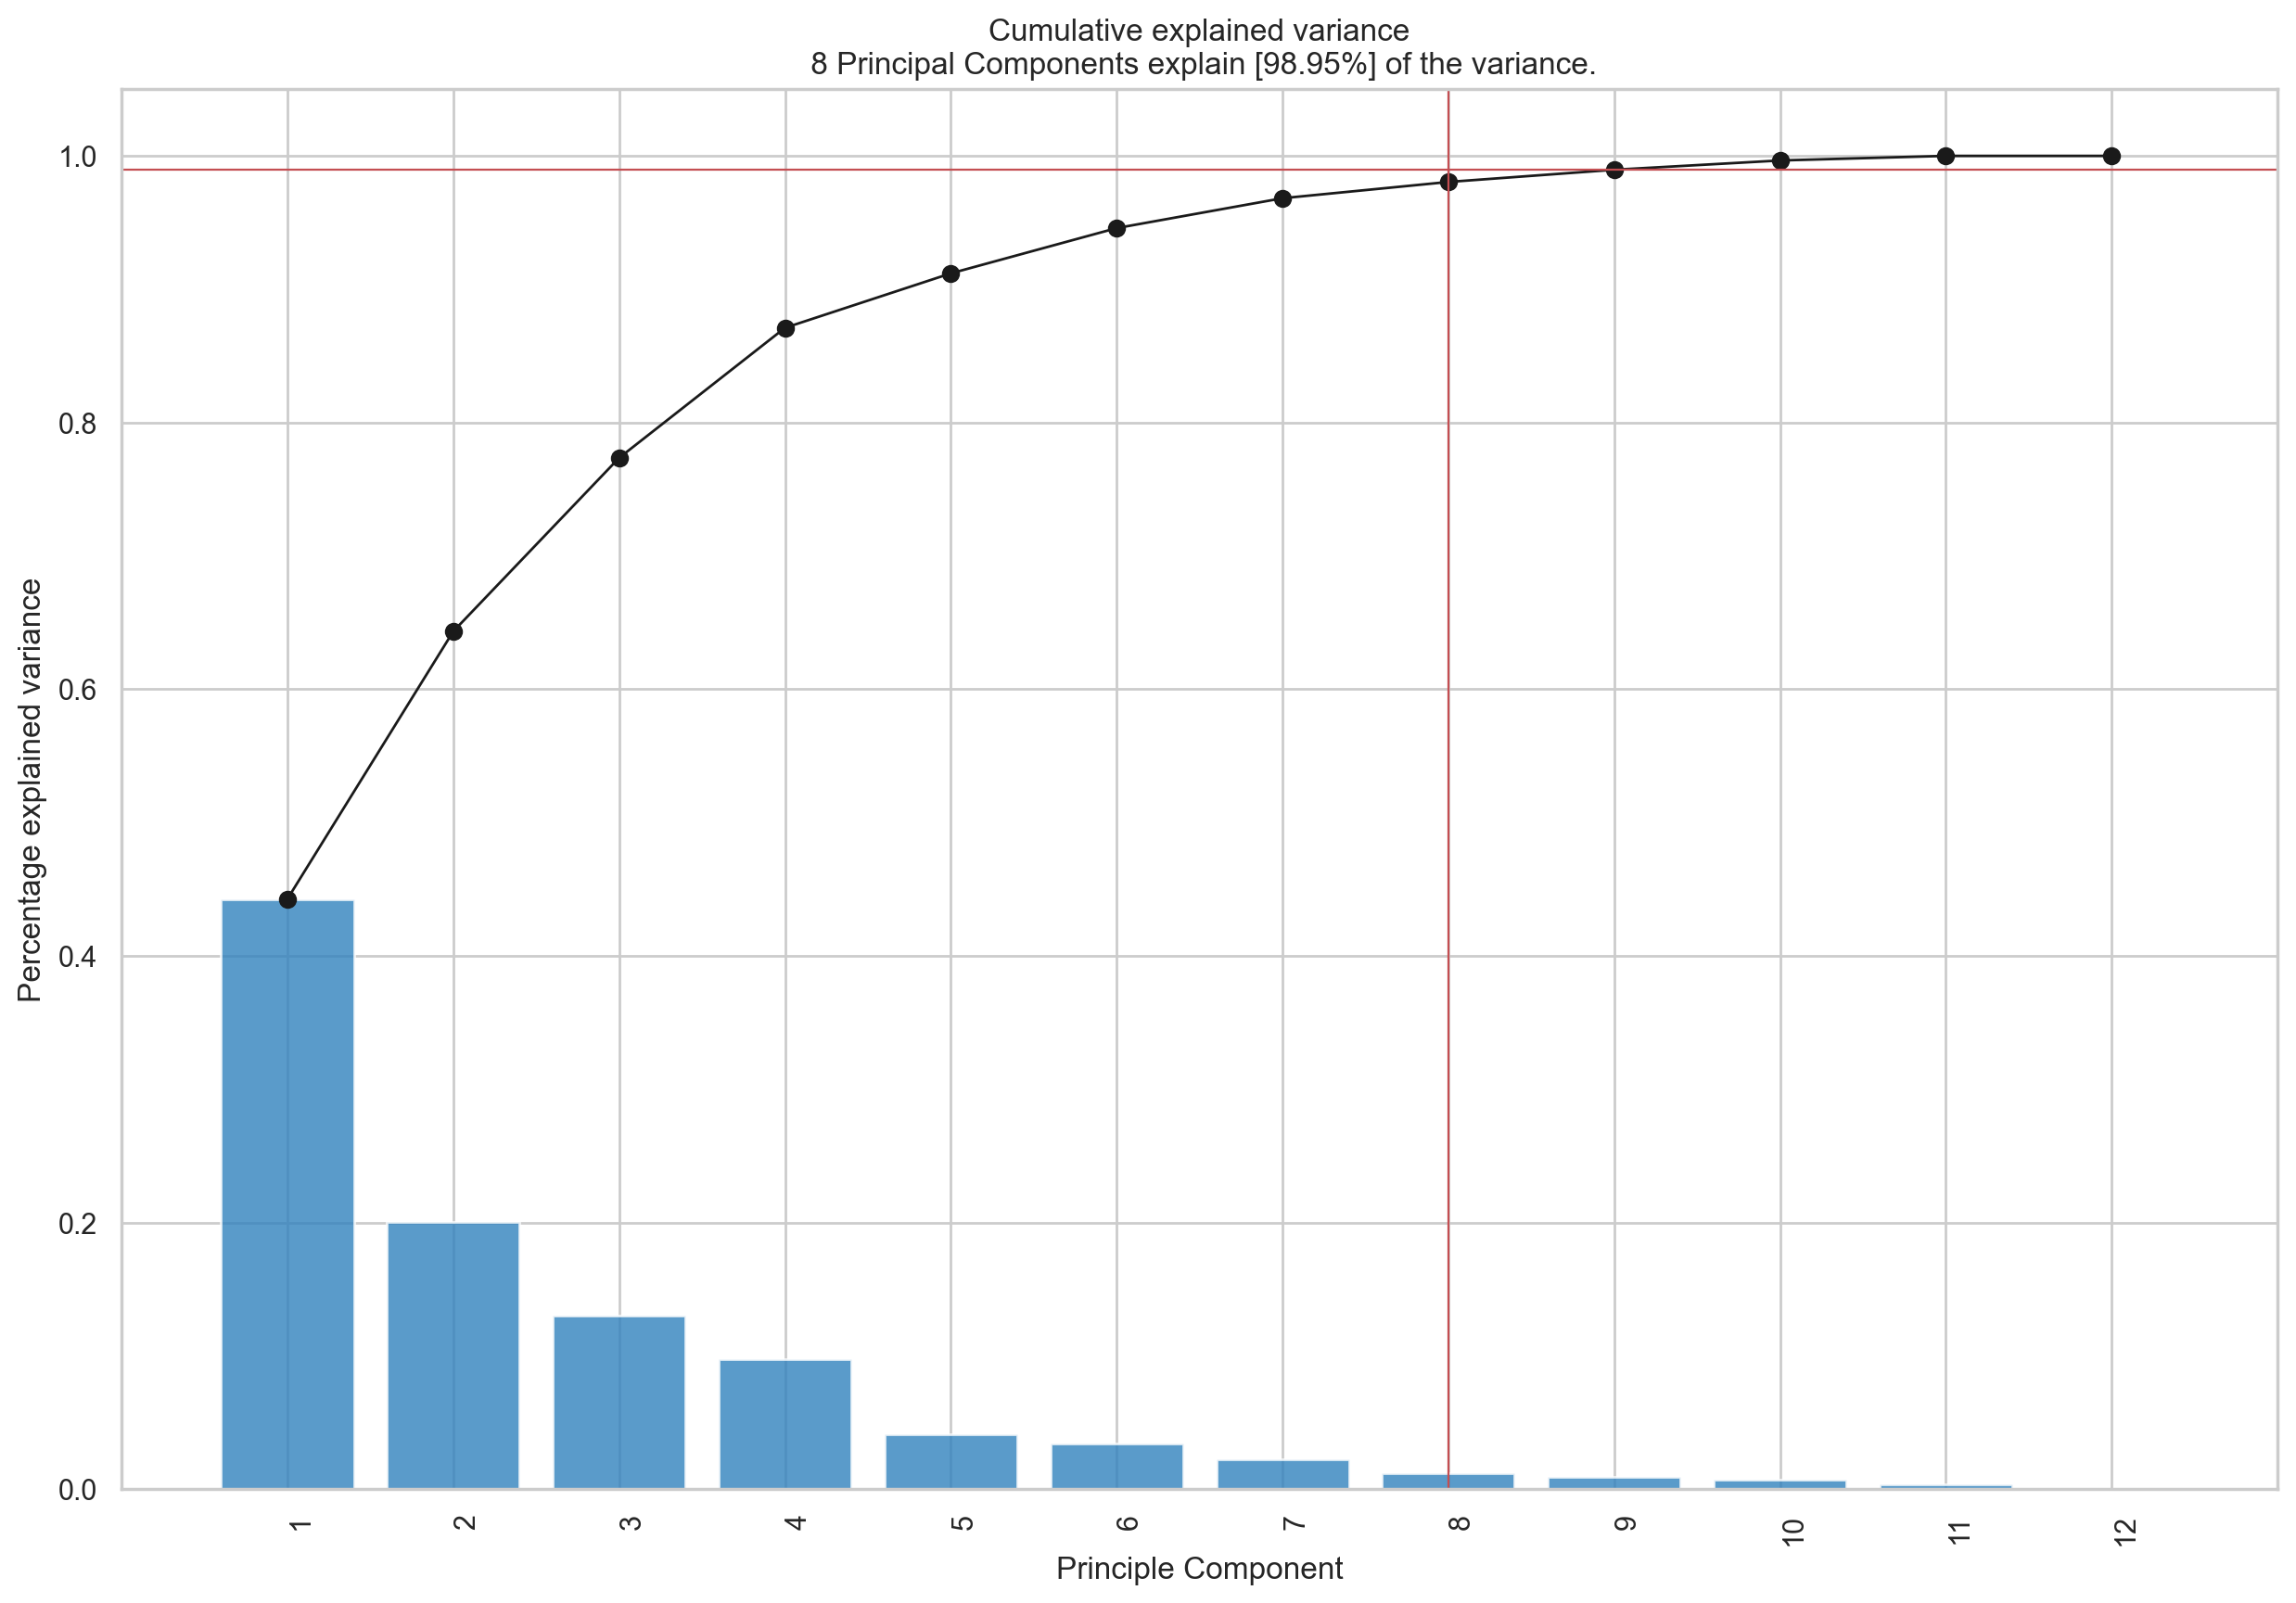
\includegraphics[width=\linewidth]{Fig1a-PCA.png}
  \caption{PCA analysis on the features. The red horizontal line is the 99\% explained variance}
  \label{PCA}
  \Description{PCA analysis of the features. We found if we keep 8 features we can still maintain 98\% of explained variance}
\end{subfigure}%
\begin{subfigure}{.5\textwidth}
  \centering
  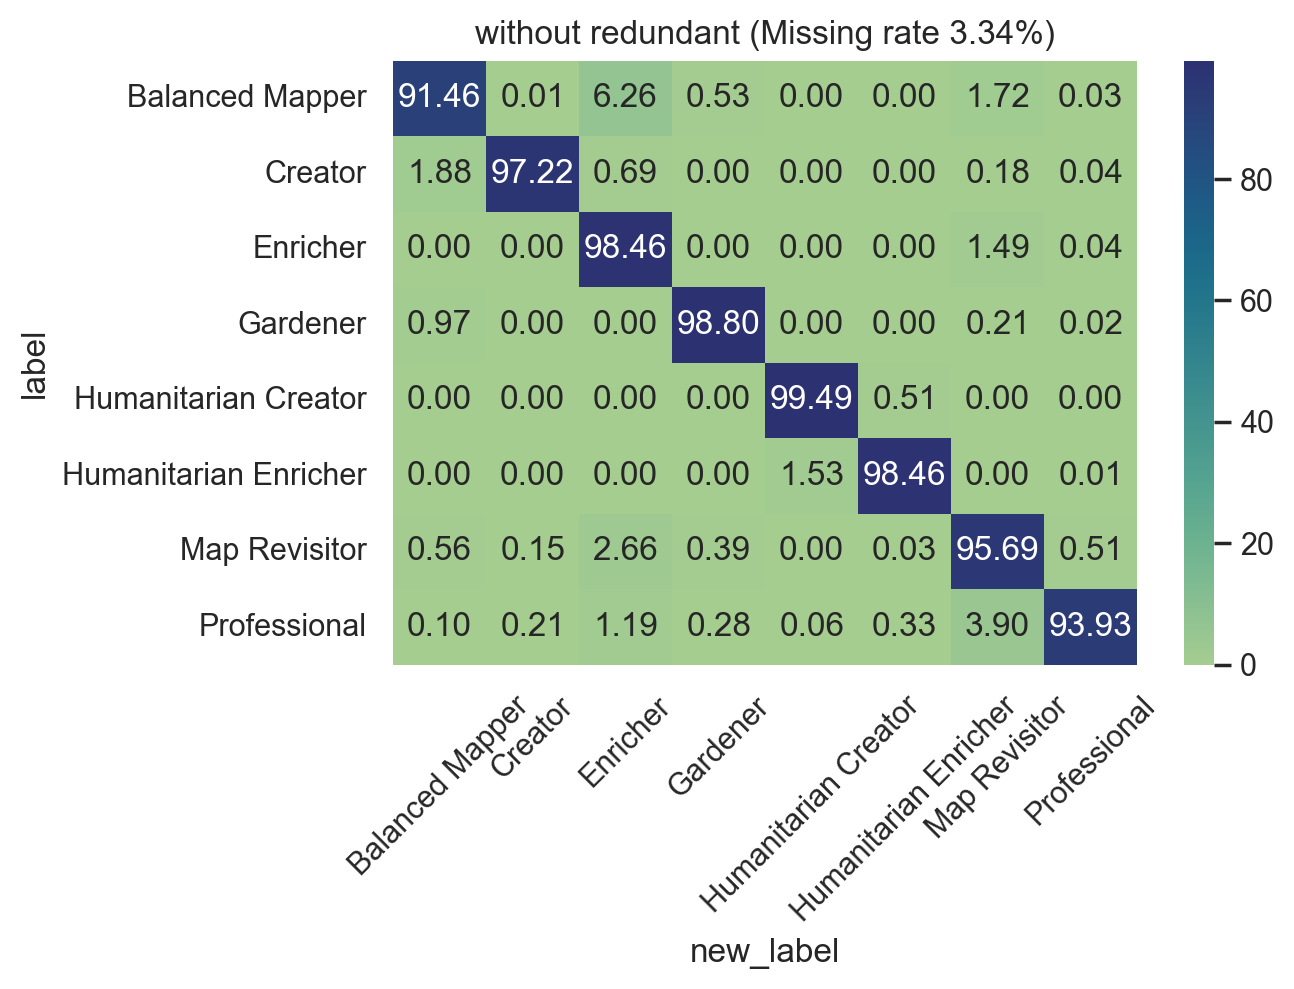
\includegraphics[width=\linewidth]{Fig1b-without redundant.png}
  \caption{Updated clustering result by excluding redundant feature}
  \label{without_redundant}
  \Description{Figure 1(b): Clustering result by excluding redundant feature. We compared the clustering before and after excluding redundant features and found a missing classification rate of 3.34\% for all the mappers and a higher than 90\% correct rate for all roles.}
\end{subfigure}
\caption{Feature reduction}
\label{Feature_reduction}
\end{figure}

To streamline our feature set and alleviate potential redundancy, we conducted Principal Component Analysis (PCA) to examine the variance explained by different feature combinations (see Fig. \ref{PCA}). The results revealed that by reducing 12 dimensions to 8, we could retain 98.95\% of the explained variance. 

To further optimize feature selection, we evaluated the impact of eliminating various feature combinations. We quantified the effectiveness of each elimination through a metric termed the "missing rate," which represents the proportion of mappers misclassified in their respective roles due to feature elimination. After extensive experimentation, we identified that excluding the features $Wh\_score$, $Country\_diversity$, $Geo\_score$, and $Value\_diversity$ resulted in the lowest missing rate of 3.34\% for role identification (see Fig. \ref{without_redundant}).

\section{Results}

\subsection{Role identification}

\begin{figure}[h!]
  \centering
  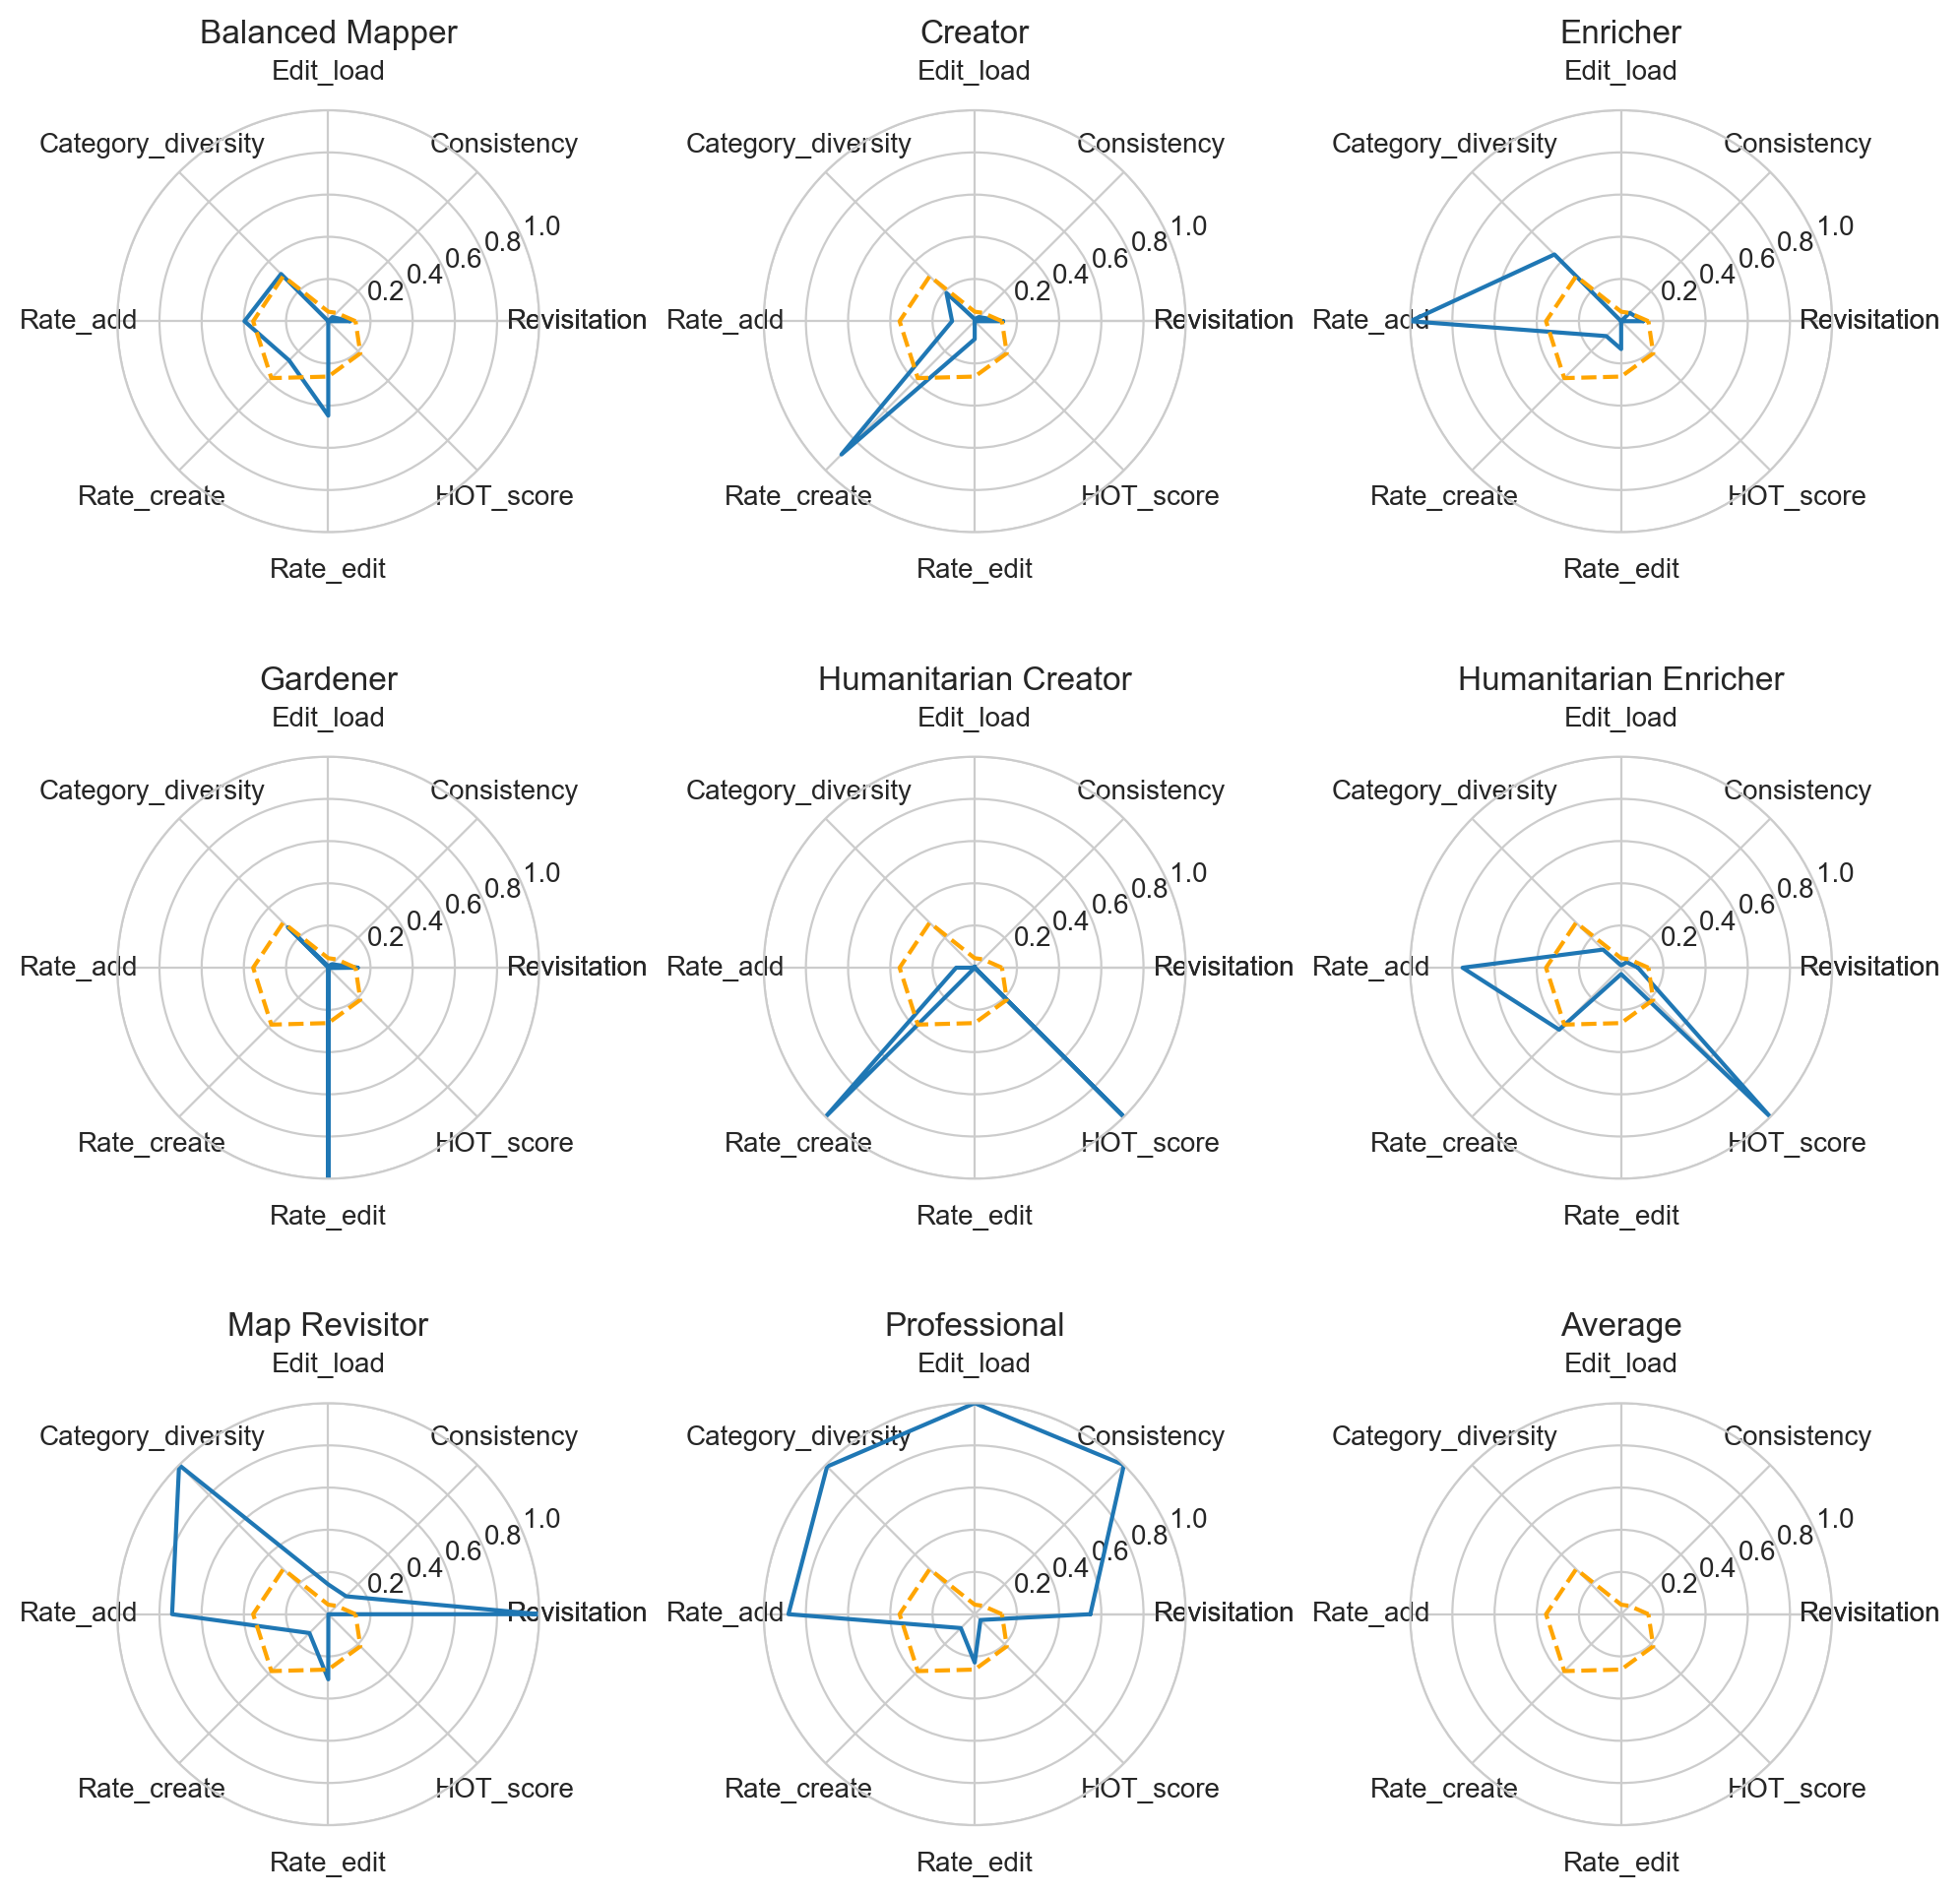
\includegraphics[width=\linewidth]{Fig2-radar_all.png}

  \caption{Radar chart for the features of mappers' features. The dashed line represents the average of the feature for all mappers}
  \Description{Radar chart for the features of mappers' features. The dashed line represents the average of the feature for all mappers. The \textbf{Gardeners}, \textbf{Creators}, and \textbf{Enrichers} are signed by their mapping type edit, creation, and add. Balanced Mappers show the most similar mapping behavior to the average. The \textbf{Humanitarian Creators} and \textbf{Humanitarian Enrichers} have high $HOT\_score$ and are classified by their mapping type. \textbf{Map Revisitors} stand out for their high revisitation and \textbf{Professionals} have high $Category\_diversity$, $Edit\_load$, and $Consistency$ compared with other roles.}
    \label{radar}
  
\end{figure}

We categorized the editing patterns into 8 distinct roles and visualized the multi-faceted editing behavior in radar charts (see Fig. \ref{radar}). In addition, we summarized the outcome of the data feature in the 4 groups we mentioned in section \ref{feature_group} in the table (see Table. \ref{table-feature}) Below is a detailed description of each role.

\begin{itemize}
\item \textbf{Balanced Mapper}: Mappers in this role demonstrate a well-balanced mapping behavior, evenly engaging in adding, creating, and editing features in OSM. Their mapping tendencies align closely with the average behavior observed across all mappers.

\item \textbf{Creator}: Mappers in this role mainly create new map features. Also, they exhibit lower-than-average mapping diversity of the different map features in OSM.

\item \textbf{Enricher}: These mappers mostly add details about existing map features and achieve a higher-than-average feature diversity in their mapping activity.

\item \textbf{Gardener}: The primary mapping behavior of these mappers revolves around editing existing map features in OSM \cite{MapGardenerMcConchie2013}. Furthermore, they exhibit a level of feature diversity in their edits that is close to the overall average observed among all mappers. Thus, unlike Enrichers, they enrich all types of OSM map features.

\item \textbf{Humanitarian Creator}: These mappers exhibit a notable inclination towards creating new map features in OSM. Additionally, they demonstrate a strong interest in humanitarian mapping endeavors while displaying a low proclivity for revisiting existing map features to enrich or improve them.

\item \textbf{Humanitarian Enricher}: Mappers in this role actively participate in humanitarian mapping efforts. However, their primary focus is on enriching existing map features by adding detailed attribute information, rather than initiating new feature creation.

\item \textbf{Map Revisitor}: These mappers are characterized by their highly diverse mapping activities and exhibit the highest revisitation rate to existing map features to add new details. 

\item \textbf{Professional}: These mappers boast the highest average edit load and engage in a high volume of mapping activities. They also display considerable diversity in the types of features they map. Moreover, they map consistently over time and maintain a strong revisitation rate.
\end{itemize}

\begin{table}[h!]
\centering
\begin{tblr}{
  width = \linewidth,
  colspec = {Q[150]Q[110]Q[110]Q[110]Q[300]},
}
& Temporal \newline Features & Edit type \& \newline \textit{Humanitarian Mapping} preferences & Feature Diversity    & Role Portrait                               \\

\textbf{Balanced Mapper}       & Average \newline Average & None \newline \textit{Low} & Low  & Balances mapping behavior between adding, creating, and editing features, contributing to the overall stability and diversity of OSM.  \\

\textbf{Creator}           & Low \newline Low & Creation \newline \textit{Low} & Low & Primarily creates new mapping features, enriching OSM with fresh geographic information beyond humanitarian efforts.  \\

\textbf{Enricher}        & Low \newline Low & Adding \newline \textit{Low} & Medium & Adds diverse elements based on existing mapping features, enhancing the richness and granularity of OSM data.  \\

\textbf{Gardener}                & Low \newline Low & Edits \newline \textit{Low} & Low  & Edits existing mapping features, ensuring accuracy and completeness of OSM data in local regions.  \\

\textbf{Humanitarian Creator}        & Low \newline Low & Creation \newline \textit{High} & Low & Creates new mapping features with a focus on humanitarian mapping, contributing to OSM's capacity for disaster response and relief efforts.   \\

\textbf{Humanitarian Enricher} & Low \newline Low & Adding \newline \textit{High} & Low & Supports humanitarian mapping projects while focusing on enriching existing features, and advancing OSM's data quality and detail.\\

\textbf{Map Revisitor}            & High \newline Low & Adding \newline \textit{Low} & High & Highly diverse and revisiting mapper, enriching OSM with dynamic and ever-evolving geographic information worldwide. \\

\textbf{Professional}         & Medium \newline High & Adding \newline \textit{Low} & High & Engages in extensive and consistent mapping with high feature diversity, contributing substantial data to OSM's global coverage. 
 
\end{tblr}
\caption{Table for behaviors on features by the mapper in roles. The "High", "Medium", and "Low" are from the comparison of behavior in the features by the roles}
\Description{Table for behaviors on features by the mapper in roles. We summarized the behavior of the roles we found in the radar chart and listed the portrait of the roles in reality.}
\label{table-feature}
\end{table}

\subsection{Distribution of the mappers by role}
\label{Distribution}

\begin{figure}[h!]
\centering
\begin{subfigure}{.5\textwidth}
  \centering
  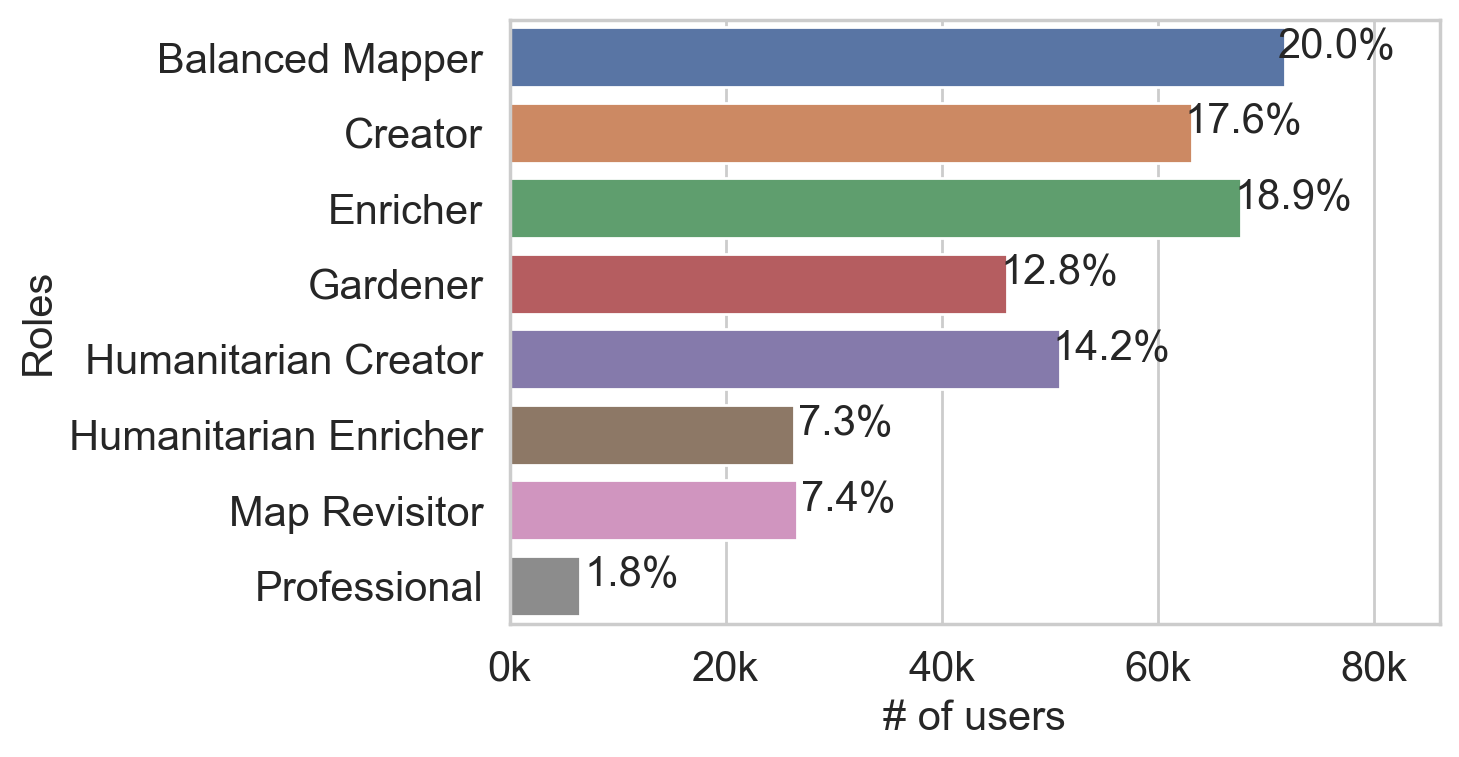
\includegraphics[width=\linewidth]{Fig3a-bar_usr.png}
  \caption{Role distribution in all mappers}
  \Description{Role distribution in all active mappers. \textbf{Balanced Mappers}, \textbf{Creators}, and \textbf{Enrichers} are the roles with the top 3 populations, which summed up over 55\%. The \textbf{Professionals} and \textbf{Map Revisitors}, on the opposite, make up only 9.2\% of the population.
}
  \label{bar_usr}
\end{subfigure}%
\begin{subfigure}{.5\textwidth}
  \centering
  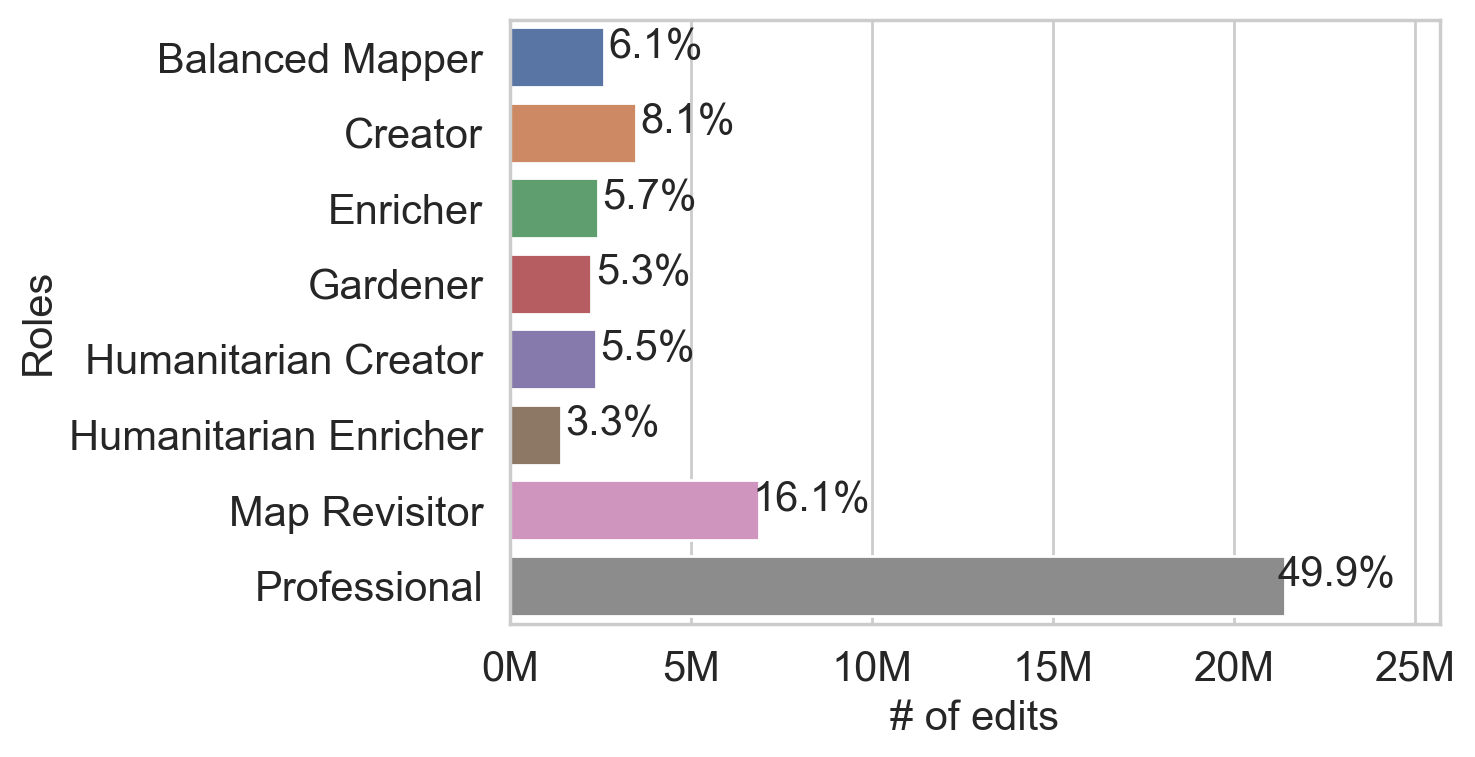
\includegraphics[width=\linewidth]{Fig3b-bar_edit.png}
  \caption{Edit distribution among all mappers}
  \Description{Edit distribution among all active mappers. The \textbf{Professionals} and \textbf{Map Revisitors} contribute over 65\% of all edits, while \textbf{Balanced Mappers}, \textbf{Creators}, and \textbf{Enrichers} contribute less than 20\%.}
  \label{bar_edit}
\end{subfigure}
\caption{Distribution of roles among active mappers}
\label{Dist_all}
\end{figure}

We found that the \textbf{Balanced Mapper} (20.0\%), \textbf{Enricher} (18.9\%), and \textbf{Creator} (17.6\%) were the top three roles among mappers (see Fig. \ref{bar_usr}). However, they only contributed around 20\% of edits. \textbf{Professional} (1.8\%) and \textbf{Map Revisitor} (7.4\%) had the most edits in OSM, contributing over 65\% of edits by around 10\% population(see Fig. \ref{bar_edit}).

\section{Insights based on role analysis}

\subsection{Mapper retention} \label{Retention}

\begin{figure}[h!]
  \centering
  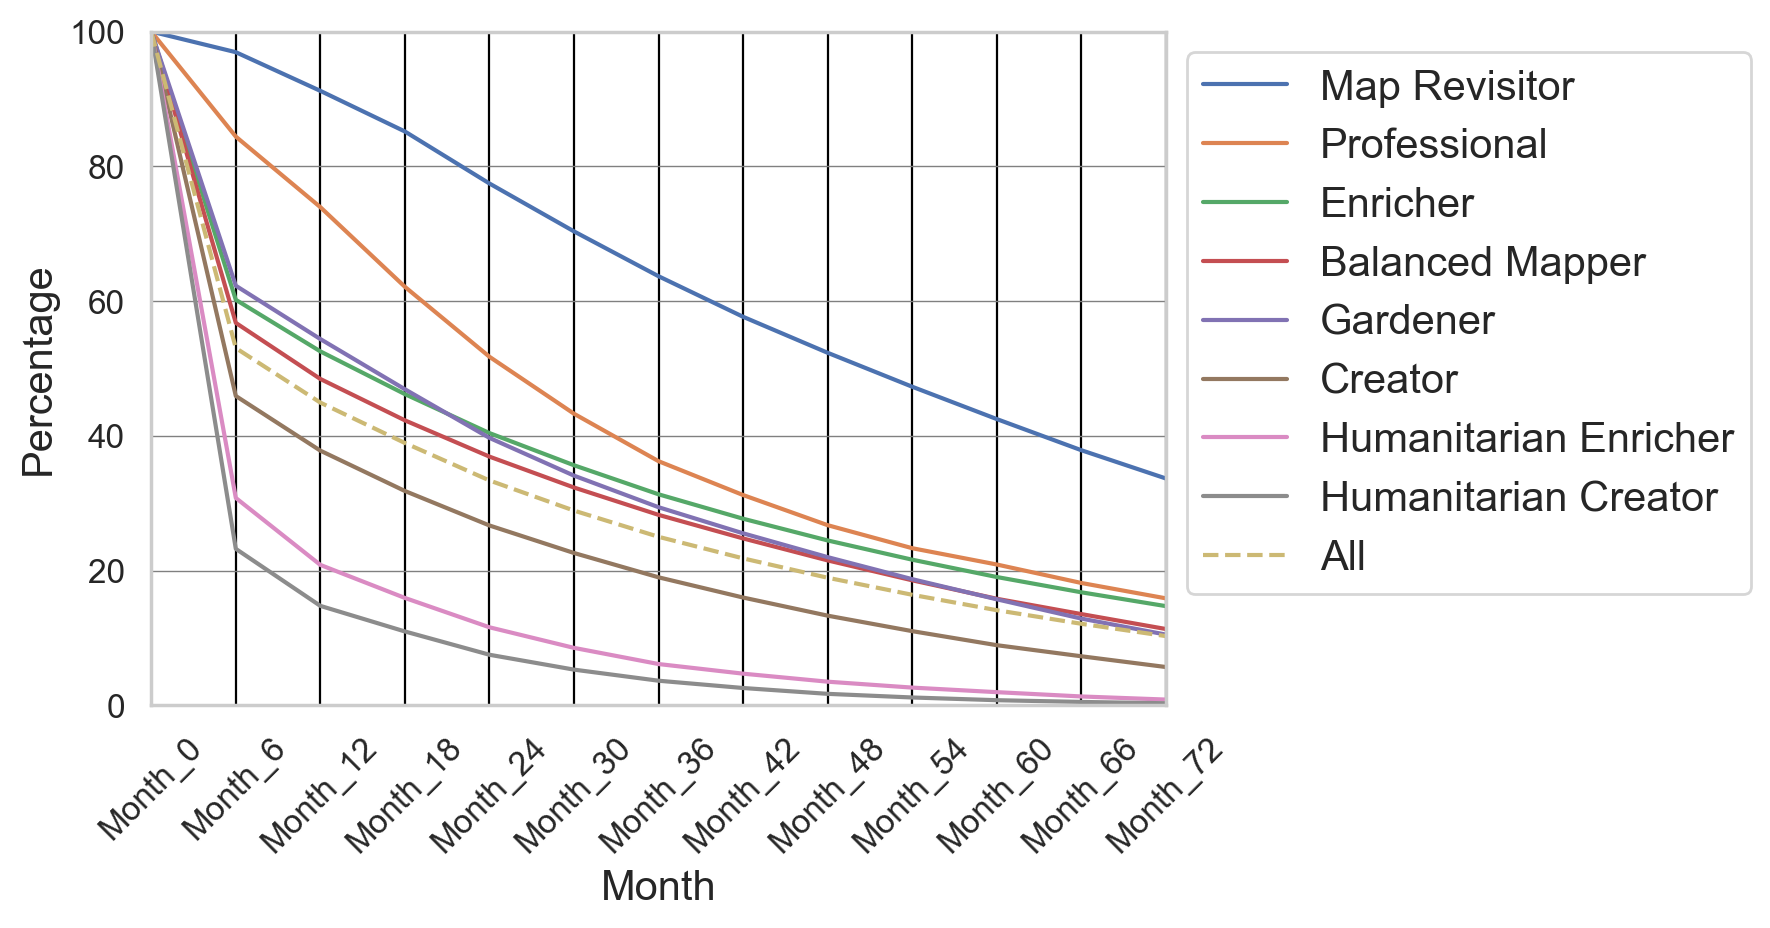
\includegraphics[width=\linewidth]{Fig4-survival.png}
  \caption{Retention of the mappers in each role}
  \Description{Retention of mappers in each role. Map Revisitors have the highest retention and the Humanitarian mappers consistently have the lowest.}
  \label{survival}
\end{figure}

To assess the retention of mappers in OSM, we conducted an analysis of continued mapping activity after an initial edit in OSM. To determine the cut-off point for evaluating retention, we referred to a previous study\cite{BeginDR18}, which found that after the 6th year, the proportion of users dropped to 1\% of all users and 4\% of active users. In our research, we observed a decline in retention to 20\% by the 5th year, with a continuous decrease thereafter. However, it is important to note that our definition of active mappers differs from \cite{BeginDR18}. Based on our definition, which considers the proportion of mappers that are still active after the time intervals we defined.

We chose a 6-month interval to assess what proportion of mappers are still making contributions in order to evaluate the changing retention rates of different mapper roles. The retention curves(see Fig. \ref{survival}) show that all roles except \textbf{Map Revisitor} and \textbf{Professional} experience a sharp decrease to around or less than 60\% within the first 6 months. \textbf{Map Revisitor} consistently demonstrated the highest retention rate throughout the observation period, followed by \textbf{Professional} and \textbf{Enricher}.  \textbf{Professional} approached a similar retention level as \textbf{Enricher} by the 3rd year. \textbf{Gardener} and \textbf{Balanced Mapper} exhibited retention rates close to the average. On the other hand, \textbf{Creator}, \textbf{Humanitarian Enricher}, and \textbf{Humanitarian Creator} displayed lower than average retention rates among the active mappers, with \textbf{Humanitarian Enricher} and \textbf{Humanitarian Creator} reaching nearly 0\% retention by the 6th year. 

\subsection{Roles of known mappers} \label{known mappers}

In this work, we chose two distinguished mapping communities in OSM: Humanitarian mappers and corporate mappers. Specifically, our clustering approach successfully identified humanitarian mappers and found a good match of known corporate mappers with the roles.

\subsubsection{Humanitarian mappers}

\begin{figure}[h!]
\centering
\begin{subfigure}{.3\textwidth}
  \centering
  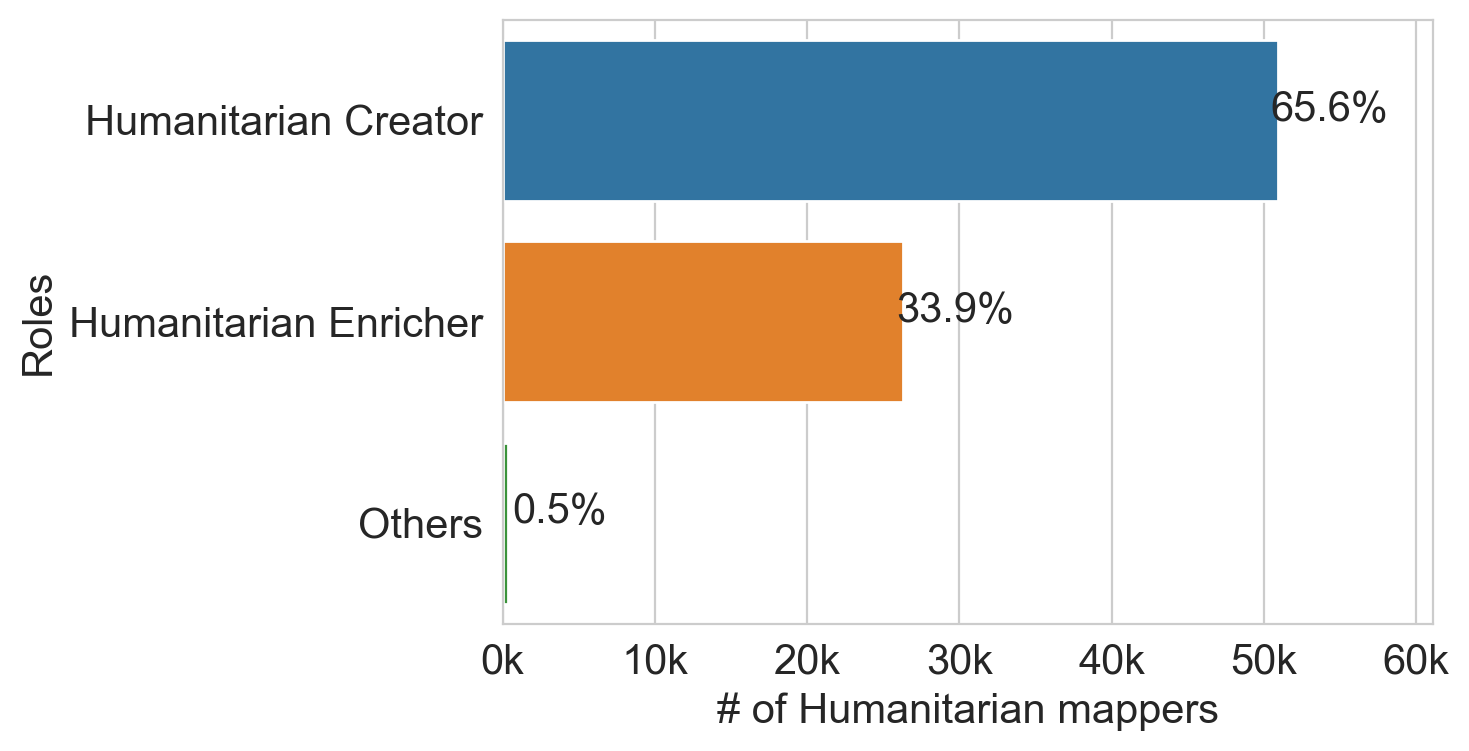
\includegraphics[width=\linewidth]{Fig5a-bar_hot.png}
  \caption{Size and percentage of humanitarian mappers of each role}
  \label{HotA}
  \Description{Size and percentage of humanitarian mappers of each role. 65.6\% of humanitarian mappers are \textbf{Humanitarian Creators}, 33.9\% of humanitarian mappers are \textbf{Humanitarian Enrichers}.}
  
\end{subfigure}%
\begin{subfigure}{.7\textwidth}
  \centering
  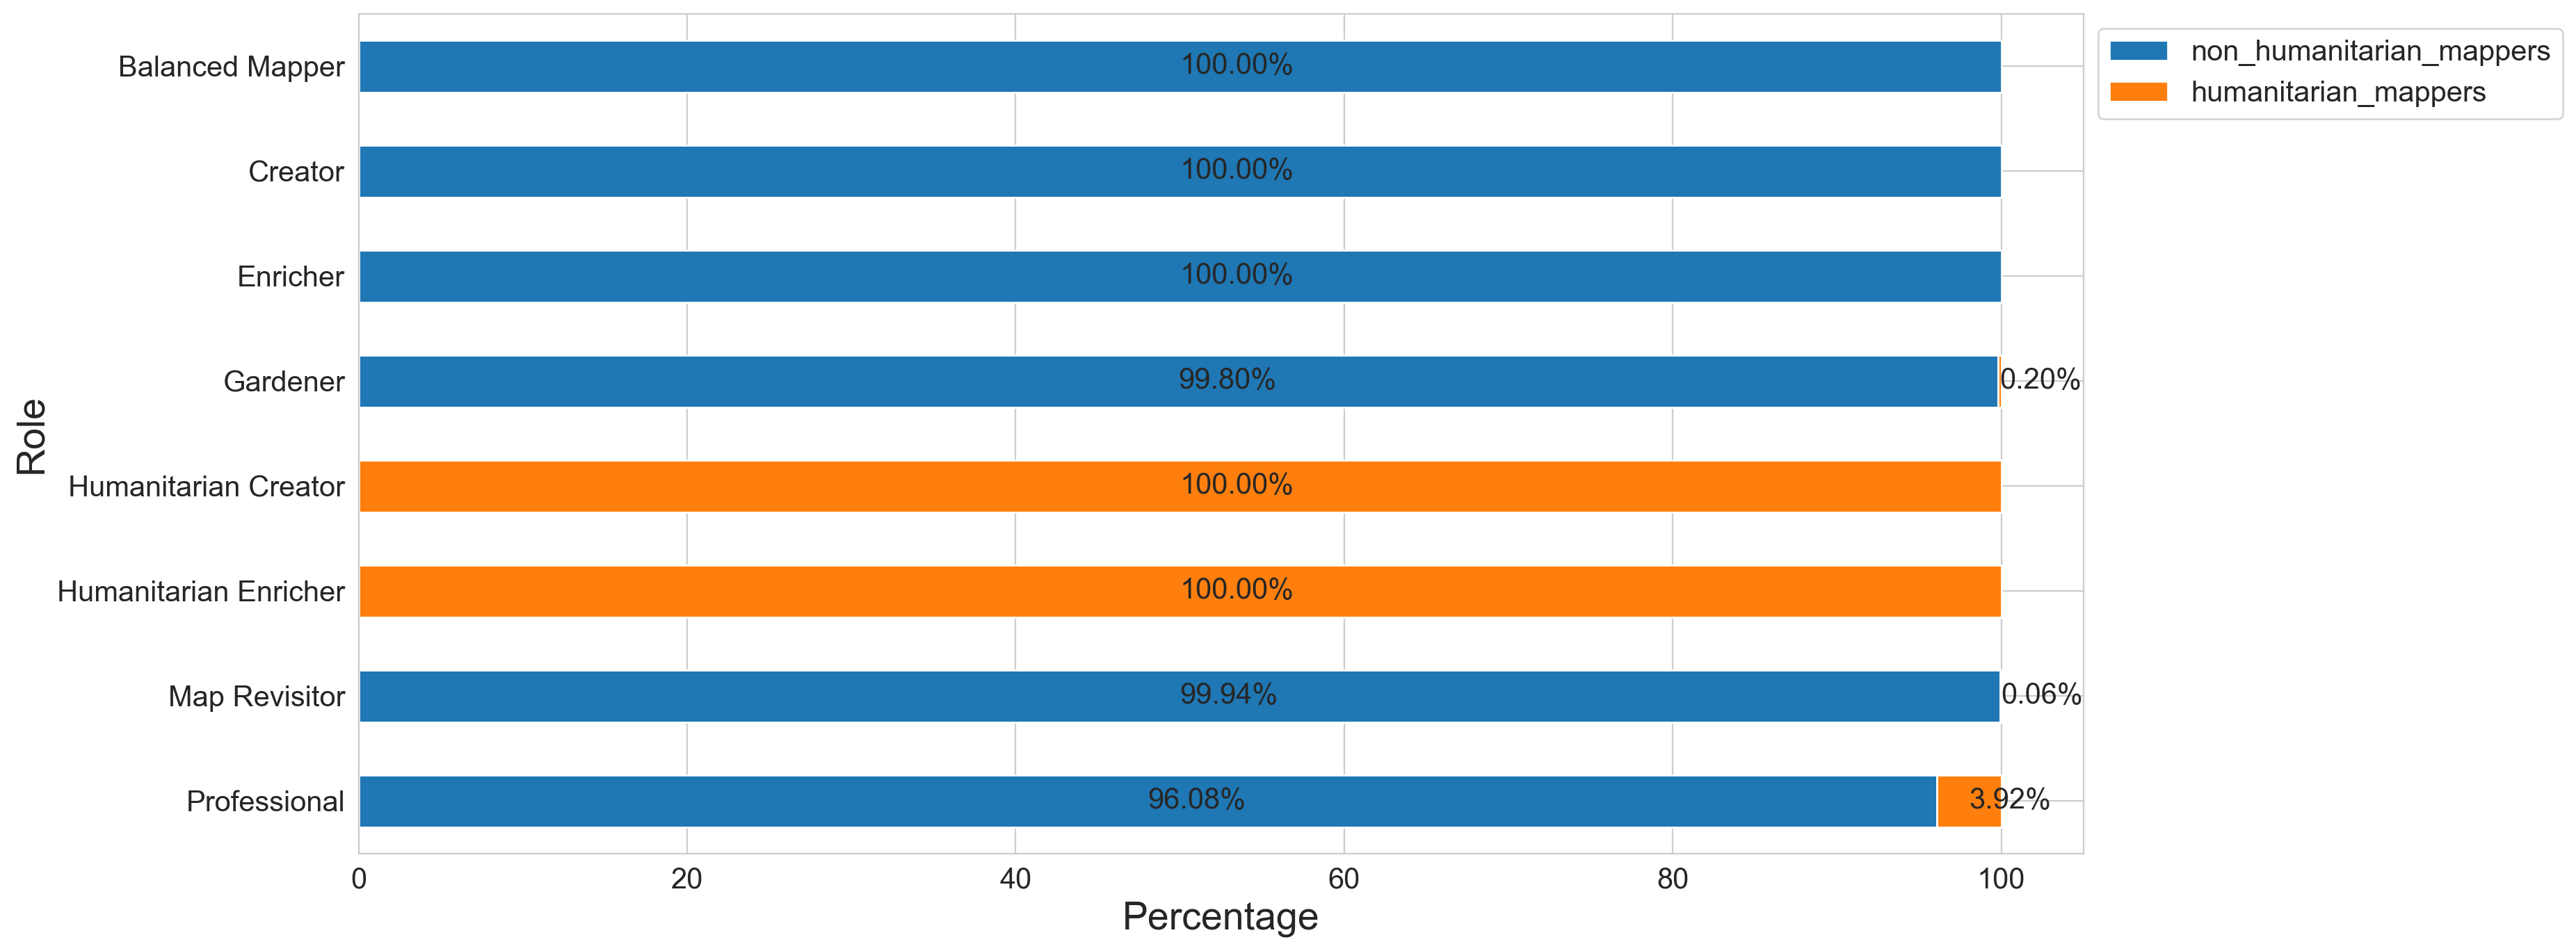
\includegraphics[width=\linewidth]{Fig5b-stack_hot.png}
  \caption{Distribution of humanitarian mappers in each role}
  \label{HotB}
  \Description{Distribution of humanitarian mappers in each role. All \textbf{Humanitarian Creators} and \textbf{Humanitarian Enrichers} are humanitarian mappers. In other roles, less than 4\% of the mappers are humanitarian mappers.}
\end{subfigure}
\caption{Roles of humanitarian mappers}
\label{Hot}
\end{figure}

Humanitarian mappers play a significant role in OSM, with many individuals introduced to the platform through their participation in humanitarian mapping projects. In this study, we identified the humanitarian mappers with 90\% of their changesets mentioning humanitarian projects in the comments or hashtags(see Fig.\ref{Hot}). Through our clustering approach, we identified two roles that are particularly associated with humanitarian mappers: the \textbf{Humanitarian Enricher} and the \textbf{Humanitarian Creator}. Among all humanitarian mappers in the data set, over 99.5\% of the mappers are correctly identified. This finding suggests that even within the humanitarian mapping community, there are distinct roles and responsibilities. Furthermore, our analysis of the distribution of humanitarian mappers revealed that approximately two-thirds of these individuals prefer to create new mapping features, while the remaining third tends to map in a more diverse range of countries.

\subsubsection{Corporate mappers}

\begin{figure}[h!]
\centering
\begin{subfigure}{.3\textwidth}
  \centering
  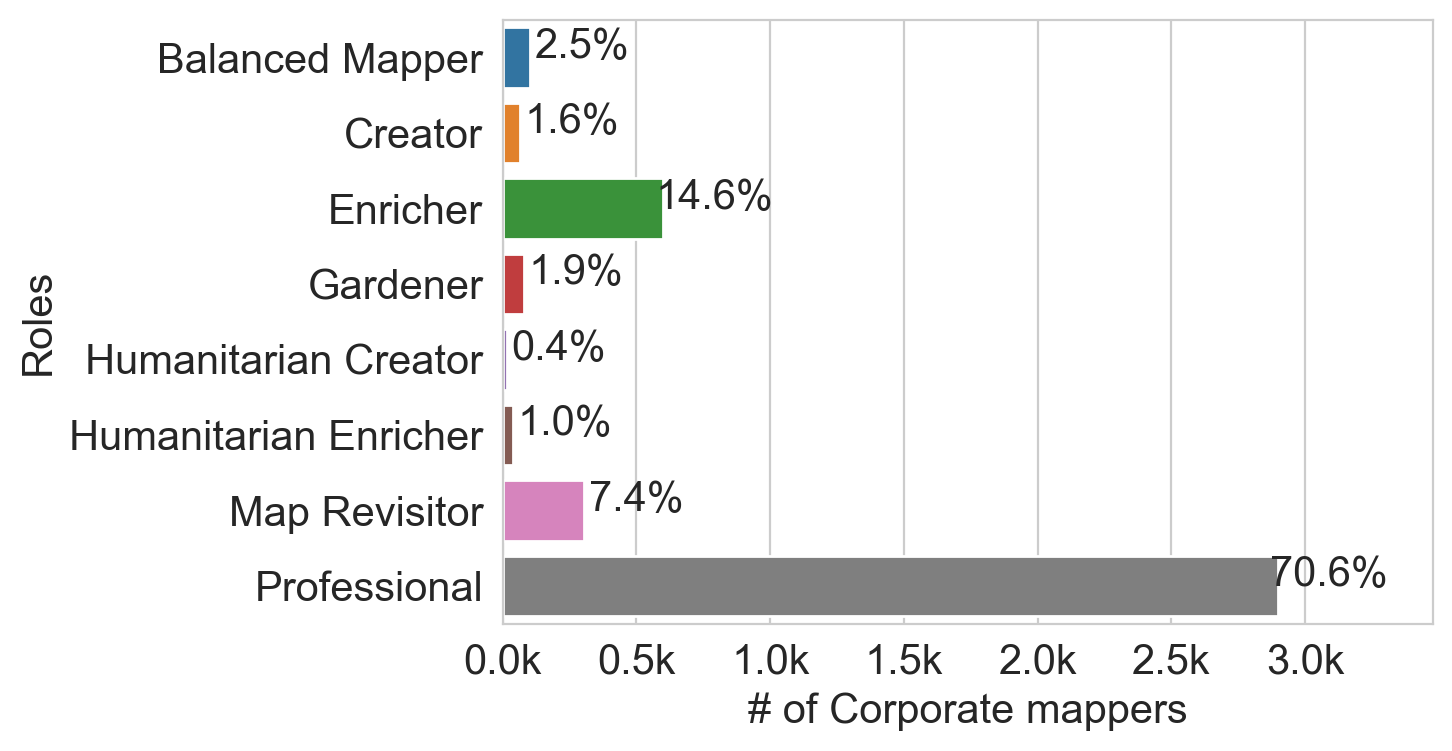
\includegraphics[width=\linewidth]{Fig6a-bar_cor.png}
  \caption{Size and percentage of corporate mappers of each role}
  \label{CorA}
  \Description{Size and percentage of corporate mappers of each role. 70.6\% of the corporate mappers are Professionals and the rest are the other roles.}
\end{subfigure}%
\begin{subfigure}{.7\textwidth}
  \centering
  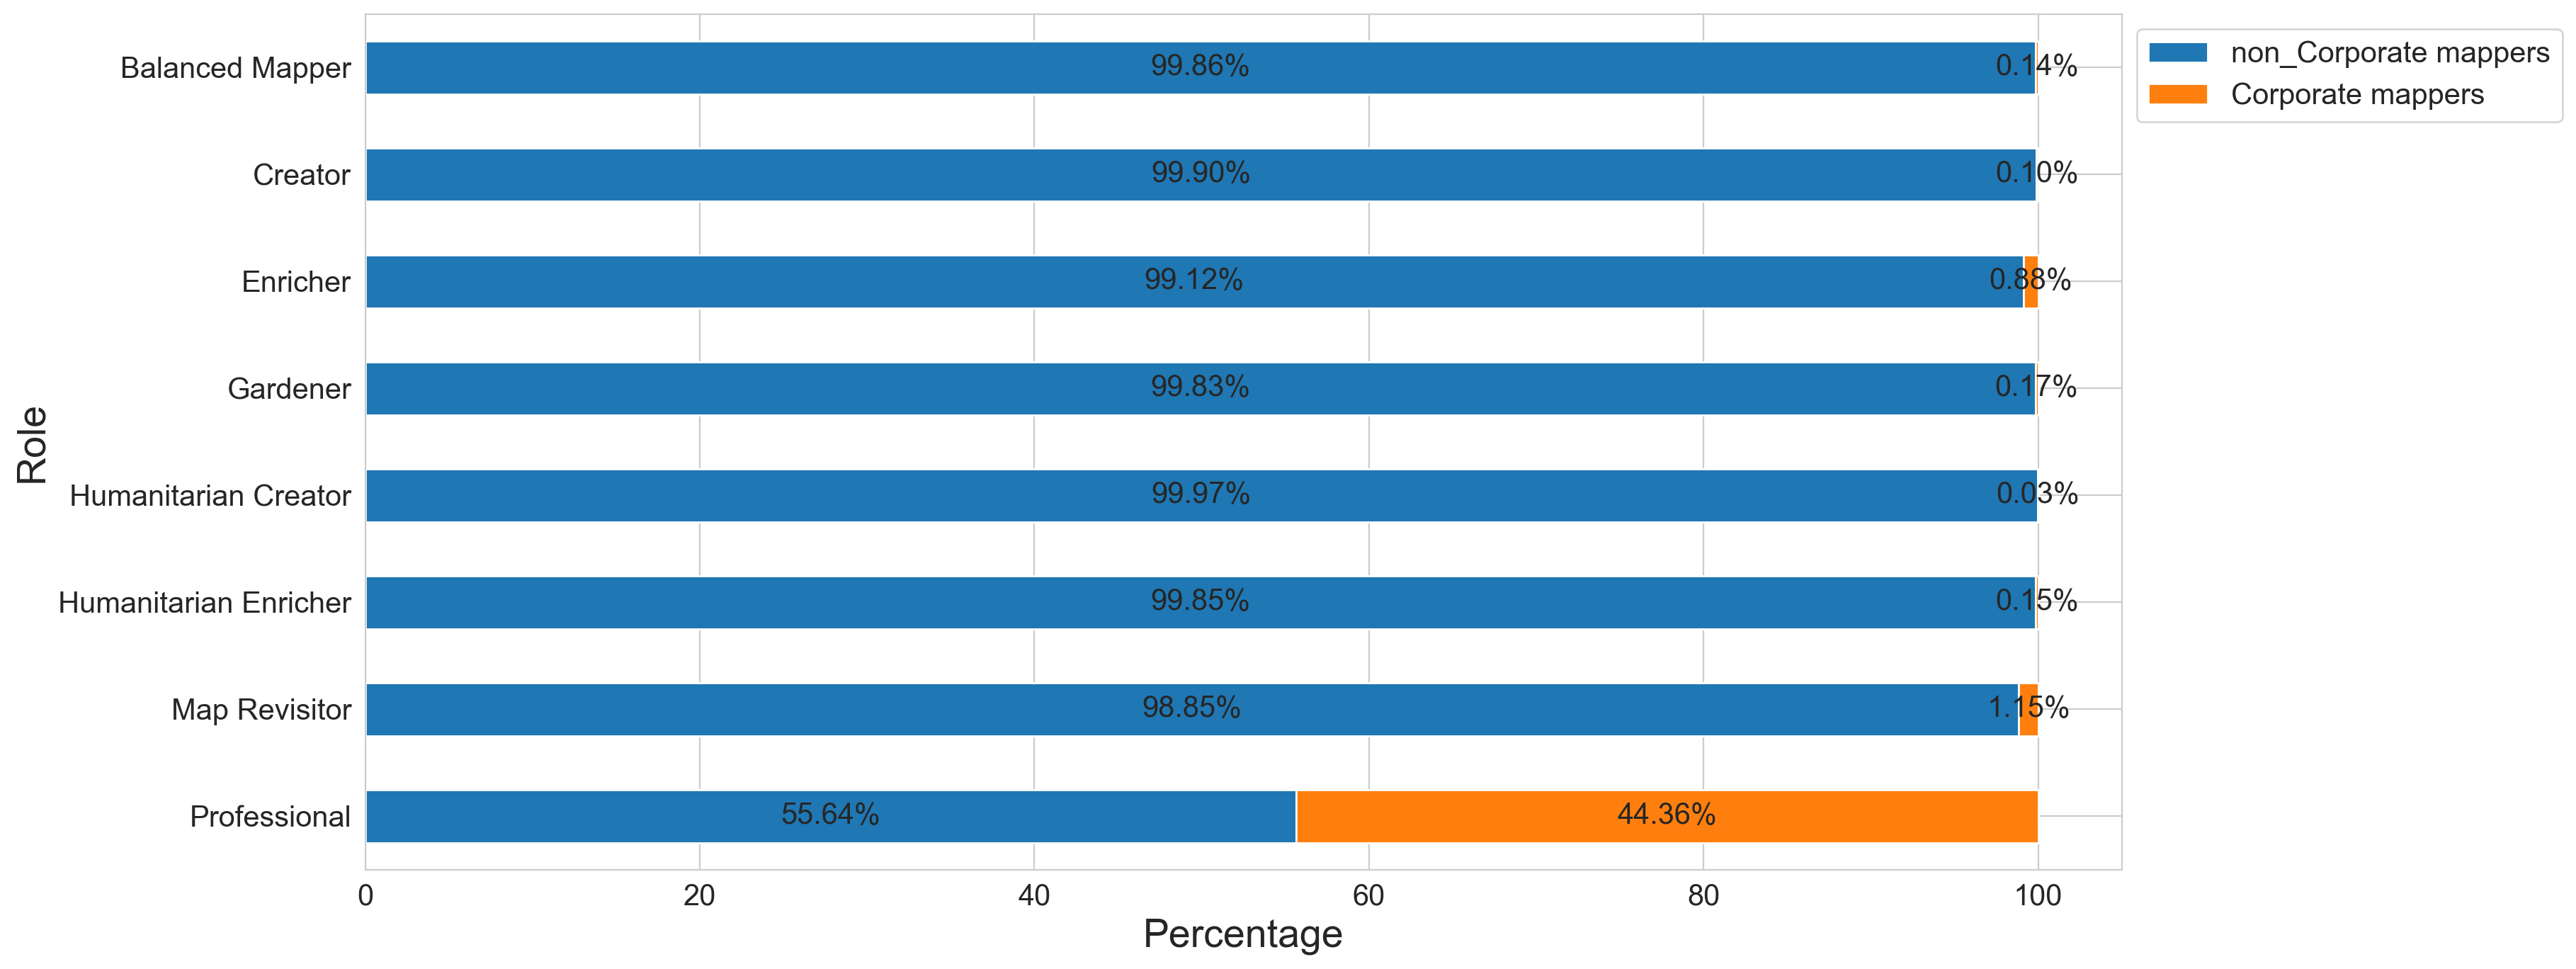
\includegraphics[width=\linewidth]{Fig6b-stack_cor.png}
  \caption{Distribution of corporate mappers in each role}
  \label{CorB}
  \Description{Figure 6(b): Distribution of corporate mappers in each role. 44.36\% of the Professionals are corporate mappers, while less than 1.2\% of the other roles are corporate mappers.}
\end{subfigure}
\caption{Roles on Corporate mappers}
\label{cor}
\end{figure}

Recent research has highlighted a growing trend of large corporations becoming involved in the OpenStreetMap community. For quantifying corporate editing in OSM, we extract a list of known mappers on the platform who self-disclosed themselves as corporate mappers.\cite{Veselovsky22} To investigate whether our identified roles contained any deterministic roles for corporate mappers, we conducted an analysis of the mapping behavior of different roles(see Fig.\ref{cor}). Our results showed that \textbf{Professional}s exhibited the closest mapping behavior to corporate mappers. Additionally, corporate mappers occupied the largest proportion of the identified roles (44.36\%), compared to less than 1.2\% in other roles. While the largest proportion of corporate mappers fell within the \textbf{Professional} category (70.6\%), the second largest group was the \textbf{Enricher}. These findings suggest that there may be a larger number of mappers who map consistently and prolifically enough to be categorized as \textbf{Professional}, but who do not work for one of the tech companies who maintain paid full-time mapping teams.

\subsection{Annual analysis of the mappers}

\label{Annual_evolution}

\begin{figure}[h!]

  \centering

  \subfloat[Active mappers each year]{
	  \label{annualA}
        \Description{Active mappers each year. Most of the time the active mappers are \textbf{Balanced Mappers} and \textbf{Enrichers}. In 2021, The \textbf{Gardener} surpassed all the roles to become the most active role.}
	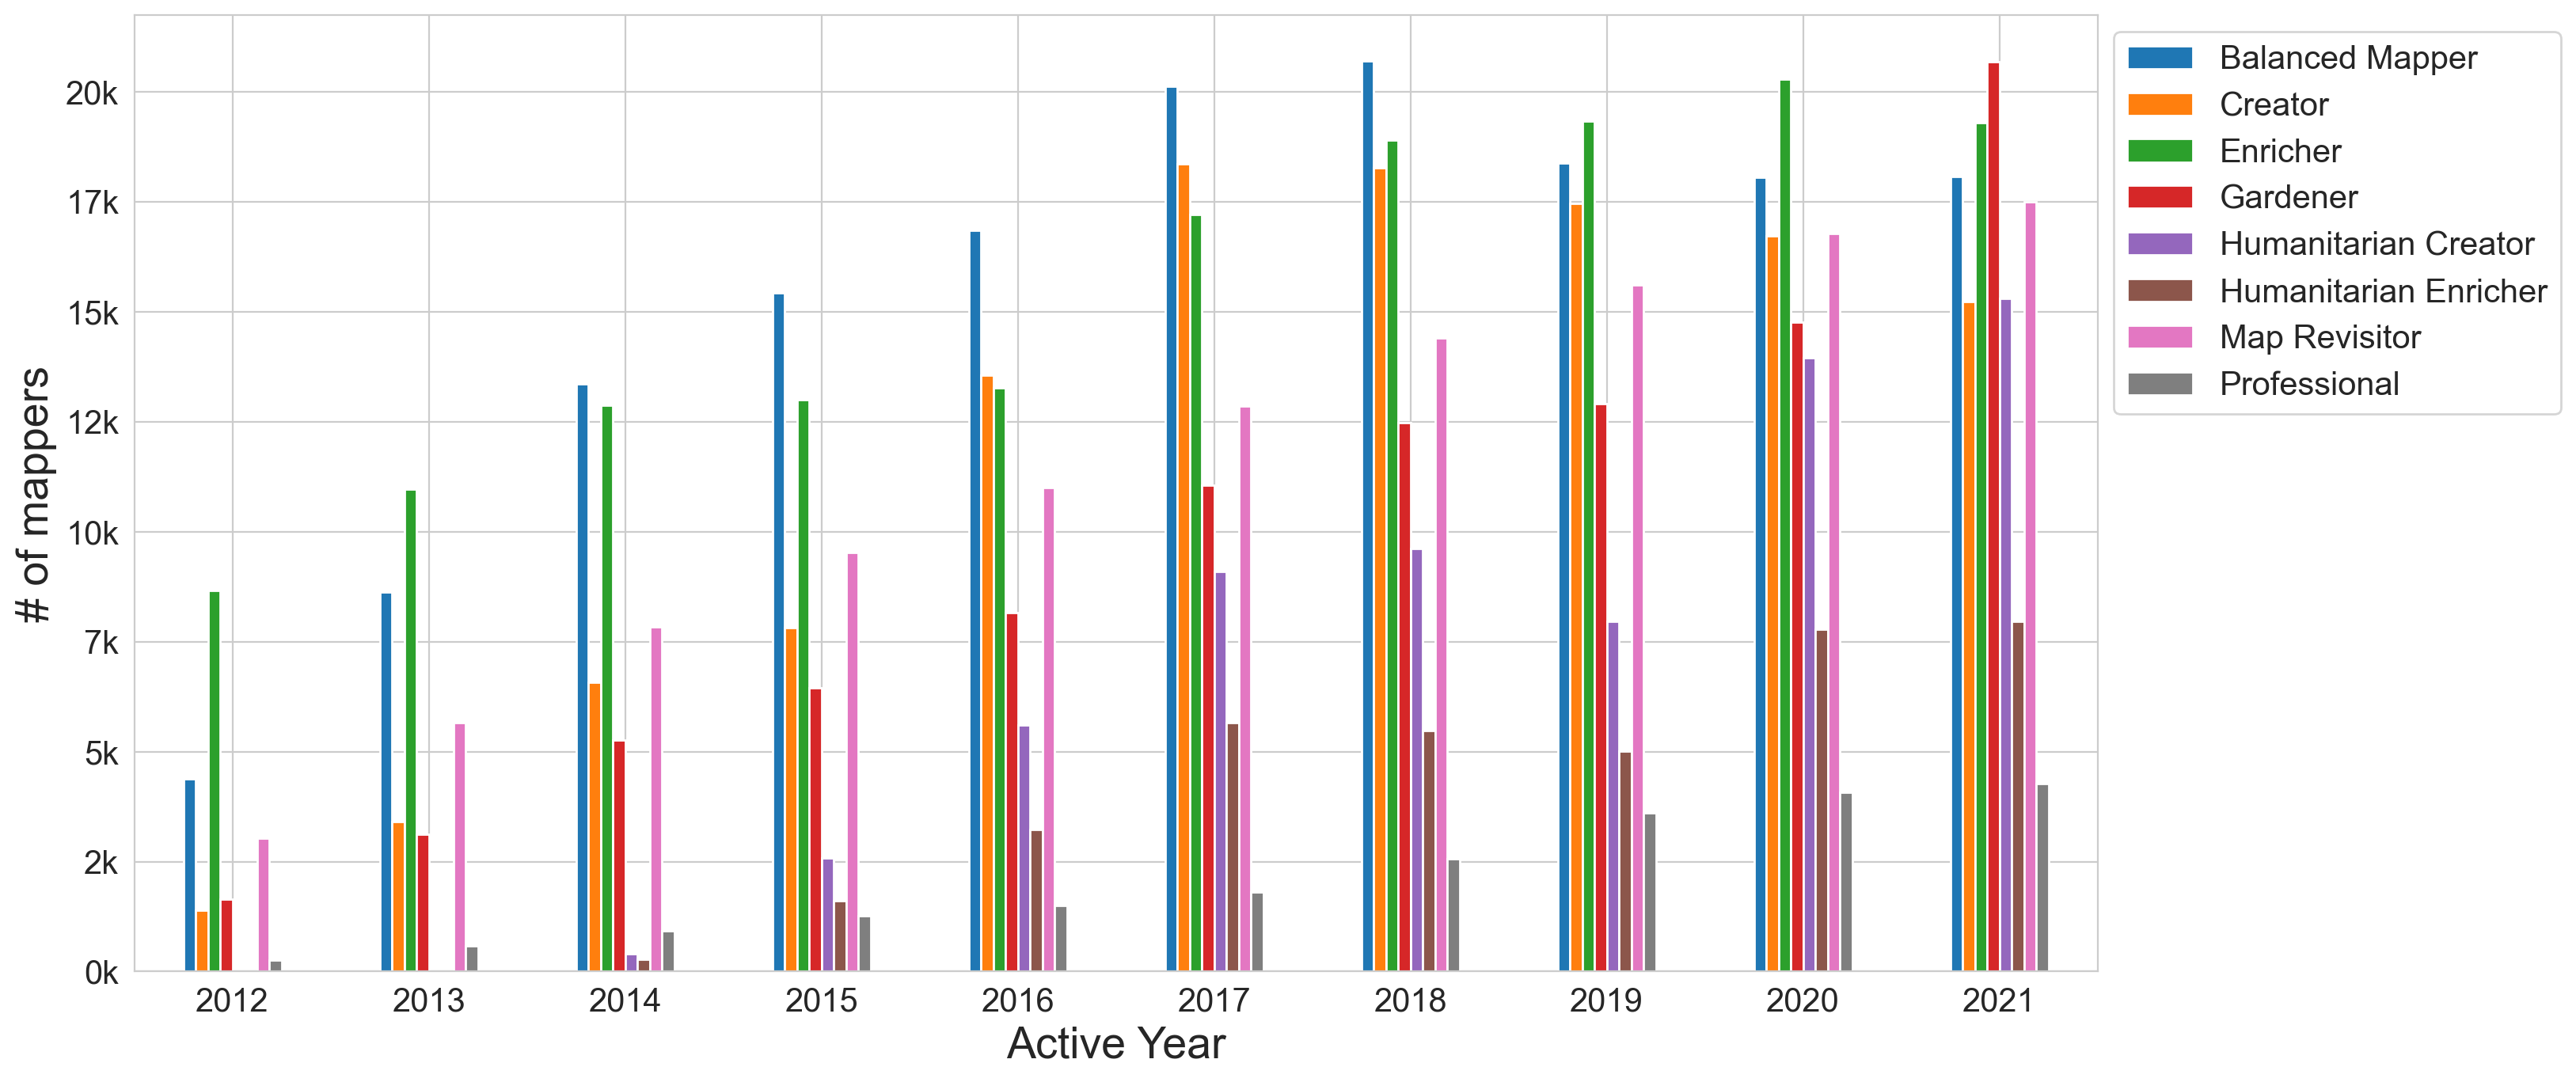
\includegraphics[width=.85\textwidth]{Fig7a-active_dist.png} }
 \hfill
  \subfloat[New mappers each year]{
	  \label{annualB}
   \Description{New mappers each year. In 2012-2015, most new mappers were \textbf{Balanced mappers} and \textbf{Enrichers}. Between 2016 and 2018, most new mappers were \textbf{Creators}. The join rate of humanitarian mappers grows consistently, topping out in 2020-2021. We also see a burst of new \textbf{Gardeners} in 2021.}
	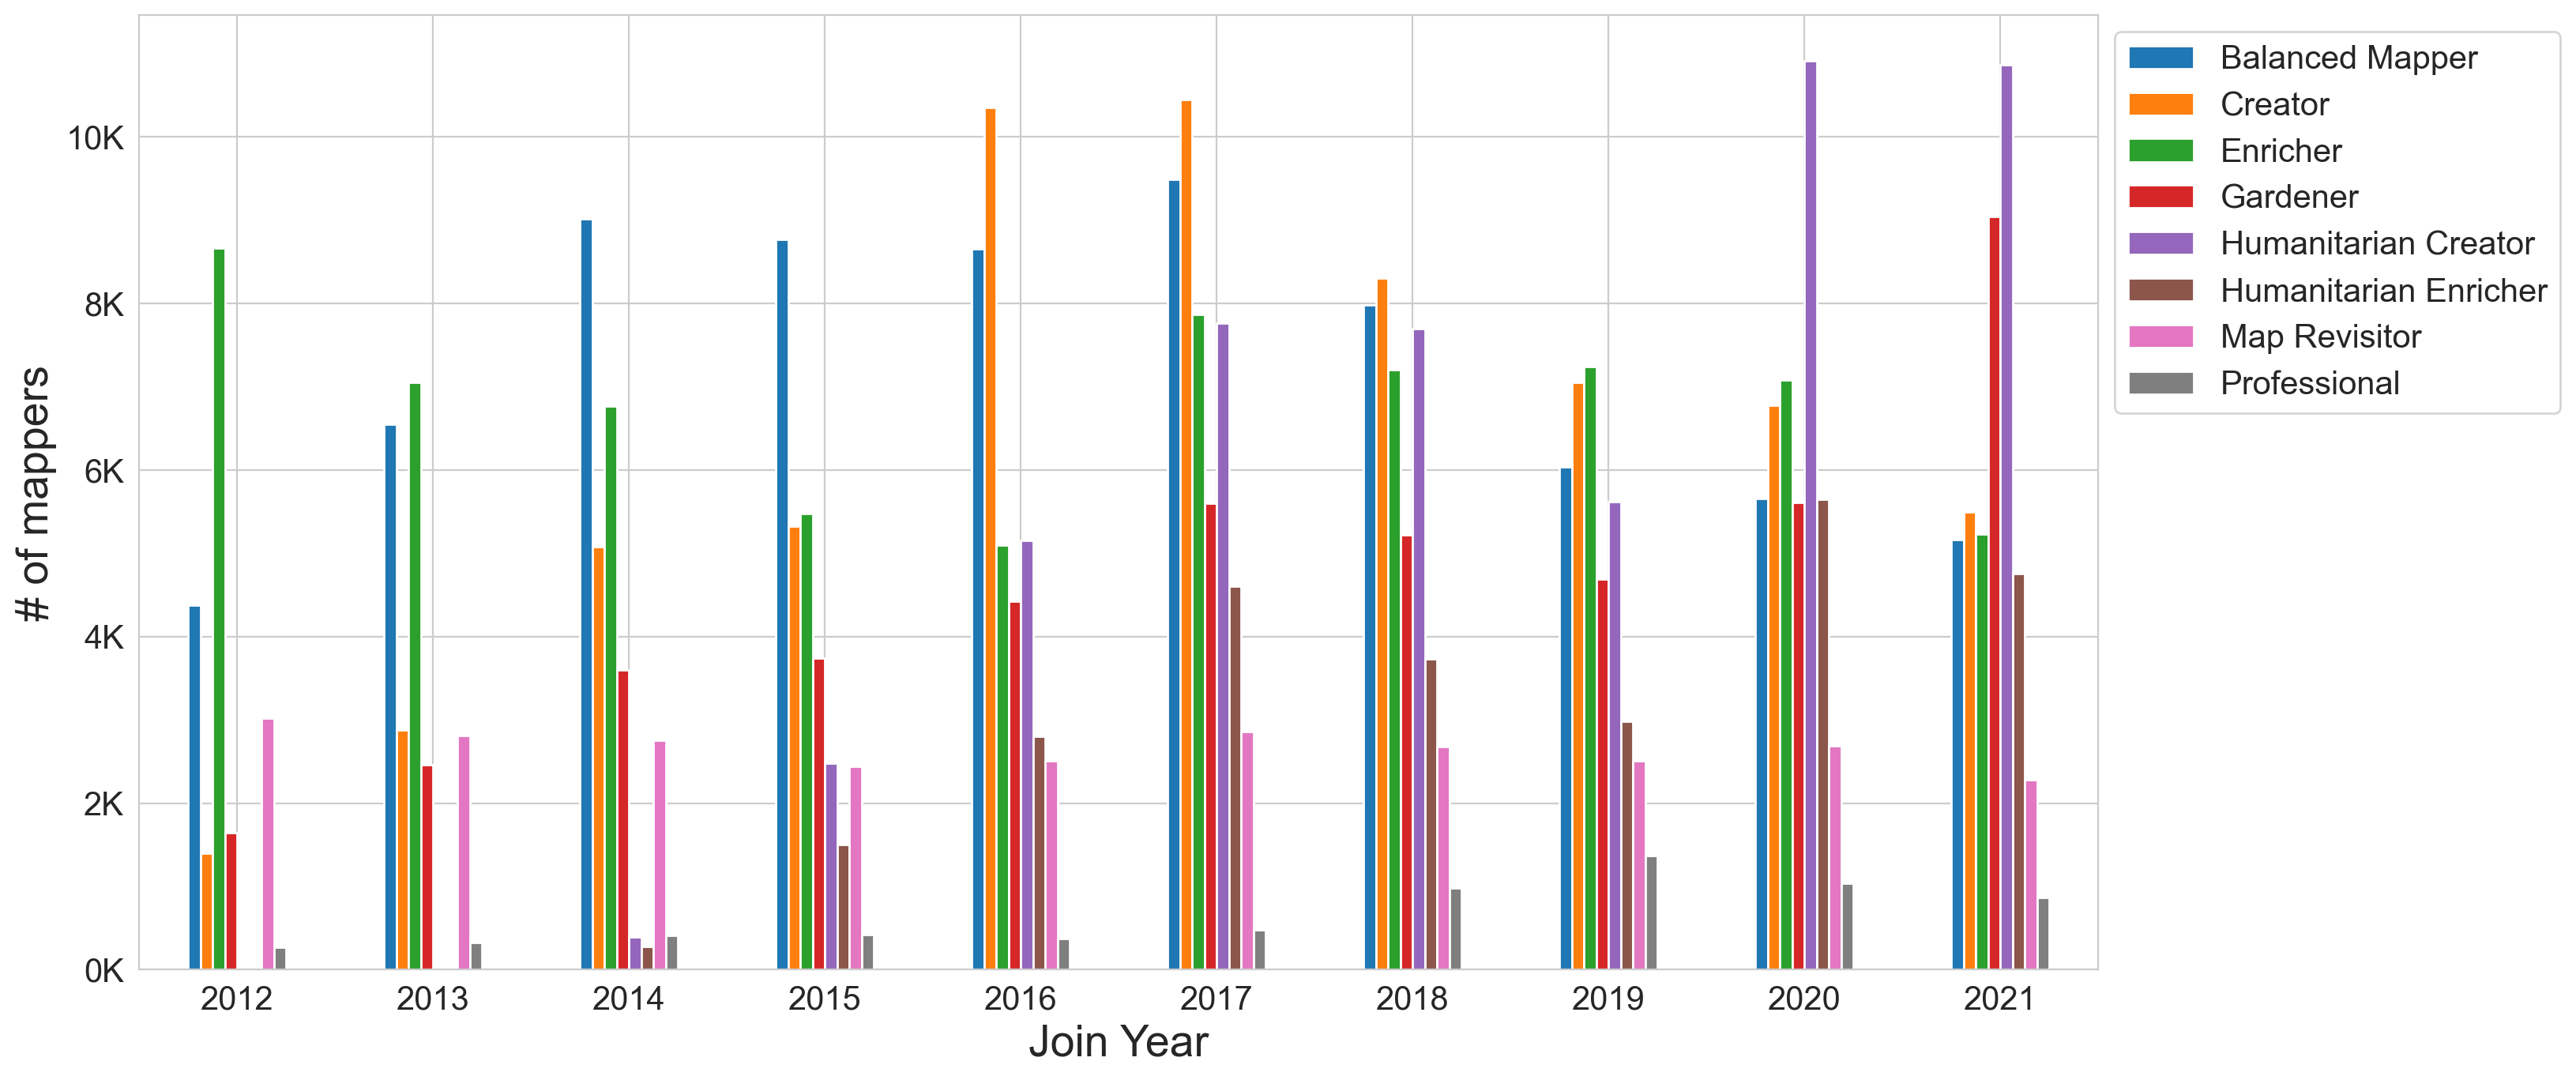
\includegraphics[width=.85\textwidth]{Fig7b-join_dist.png} } 
        
  \subfloat[Edits per role each year]{
	  \label{annualC}
   \Description{Edits per role each year. The majority of the edits are done by \textbf{Map Revisitors} and \textbf{Professionals}. The edits of \textbf{Professional} burst in 2018, peaked in 2020, and went slightly down in 2021.}
	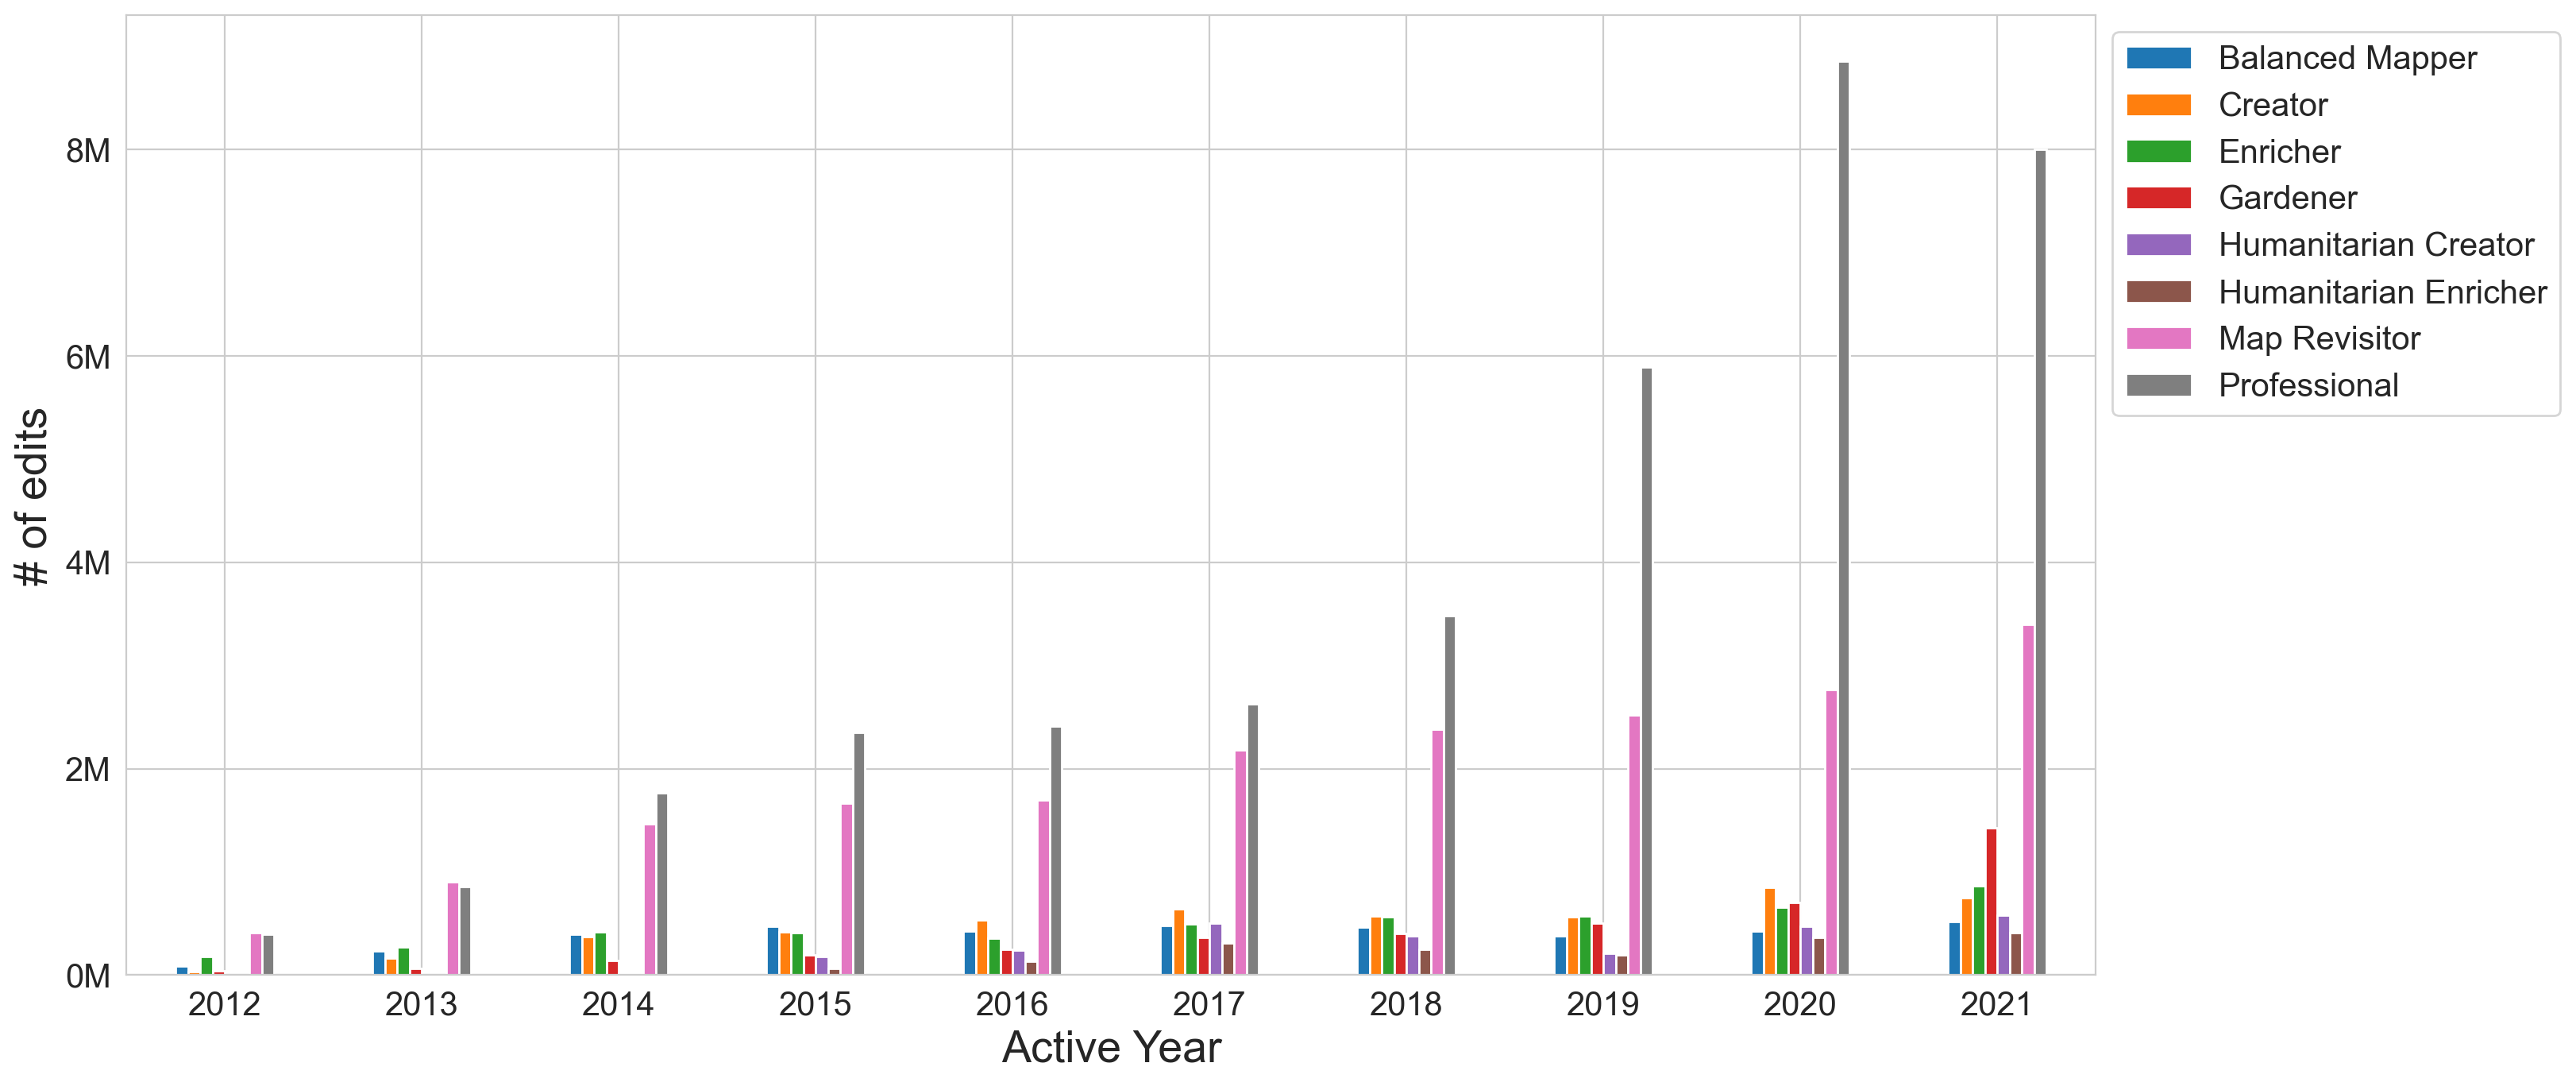
\includegraphics[width=.85\textwidth]{Fig7c-edit_dist.png} } 
        
  \caption{Active mappers, new joining mappers, and edits done by the mappers in calendar years}
  \label{annual}
  \end{figure}

The temporal evolution of user role emergence within the OpenStreetMap (OSM) community has exhibited notable dynamics, characterized by the emergence of novel roles alongside fluctuations in the prominence of existing ones (Figure \ref{annual}). In 2013, a discernible upsurge in the \textbf{Humanitarian Creator} and \textbf{Humanitarian Enricher} roles began a trend that has continued with sustained expansion over subsequent years. This growth trajectory slowed in 2019, followed by another remarkable surge in new registrations during 2020 and 2021. It is noteworthy, however, that accounts registered during this time have exhibited limited activity and contributions since.

Meanwhile, the \textbf{Enricher} and \textbf{Balanced Mapper} roles have consistently maintained their positions among the top three most active during the period spanning 2012 to 2021. This trend is further reflected in the influx of newcomers during the years 2012 to 2015, predominantly aligning with these two roles. Notably, the span from 2014 to 2017 witnessed a surge in the participation of \textbf{Balanced Mapper} individuals, who not only joined in larger numbers but also exhibited heightened engagement compared to \textbf{Enricher} mappers. Within the years 2016 to 2018, a notable influx of new mappers assumed the \textbf{Creator} role, resulting in the accumulation of active mappers that closely approximate the figures observed for \textbf{Enricher} and \textbf{Balanced Mapper} roles.

The role of \textbf{Gardener} has demonstrated a consistent trajectory of growth in terms of active mappers. Notably, the influx of new participants in this role mirrors the aggregate number of newcomers to the OSM platform during the same time span. Similarly, the \textbf{Map Revisitor} role has exhibited a steady increase in active participants, although contrasting the \textbf{Gardener}, the count of new joiners to the \textbf{Map Revisitor} role has remained relatively stable over successive years. The editing endeavors of \textbf{Map Revisitor} mappers have displayed a persistent upward trend, surpassing the growth rates observed in other roles, excluding \textbf{Professional}. The latter, characterized by remarkably heightened average mapping activities, particularly during 2019-2021, has witnessed a gradual increment in its active membership. The peak of new entrants into the \textbf{Professional} role was observed in the year 2018.

\section{Discussion}

\subsection{Methodological Considerations in the Quantitative Analysis of Peer Production Behavior}
Based on research linked to Wikipedia users, we determined that we would need to separate our changeset data in new ways than what was done in previous OSM research so that we could fine-tune mappers’ roles and activities. These changes gave us the opportunity to analyze mapper contributions more decisively. 

Our investigation into mapper roles within the OpenStreetMap (OSM) community discerned eight distinct roles defined by their distinctive mapping behaviors. First, we filtered the dataset to include only mappers with a minimum of ten contributions. This removed nearly three-quarters of the total number of mappers who collectively accounted for a mere 3\% of the entire changeset count. Upon applying the filter for active mappers, the observed distribution exhibited a distinct contrast to the overall trend, revealing a more balanced distribution of roles.

Building on prior OSM research that predominantly focused on mapper preferences at the object level \cite{Neis12}, our study drew inspiration from Wikipedia studies \cite{Yang21} and adapted its approach to the OSM context. Recognizing the prominence of changesets in OSM contributions, we extended our analysis to the changeset level. A key aspect of our methodology involved categorizing editing actions into discrete types: "edit," "add," and "creation." While Yang et al.'s investigation \cite{Yang21} on Wikipedia primarily inclined towards using reverts and deletions. A similar recent work from Neis et al.\cite{Neis23} raised a new metric of reverted mappings which would also be interesting for future research on mappers' contributions. Our comprehensive analysis of the OSM dataset identified a smaller group of mappers engaged in these specific edit types. To enhance accuracy, we consolidated changesets, excluding creations and additions, under the "edit" classification. This consolidation enabled us to distinguish mappers with distinctive preferences for specific feature categories within the mapping domain.

We also found that while the geographic location of edits often plays an important role in understanding mapping behaviors, they have minimal influence on role identification. This surprising finding prompts a deeper examination of the connection between geographic attributes and the multifaceted nature of mapper roles, further accentuating the nuanced dynamics inherent in the OSM ecosystem. Furthermore, the decentralized nature of mapping in OSM, often transpiring remotely, poses complexities in discerning whether contributions are made locally or from a distance. We improved upon \cite{Veselovsky22} method of aligning mappers' time zones with editing behavior during typical working hours to find the location of the mappers. Further exploration into mechanisms for extracting and integrating accurate geographic information, like the location of the editors, would undoubtedly improve the fidelity of our role characterizations.

We developed two features of consistency and revisitation rates to better weigh the overall temporal style the mappers are mapping in OSM. Previous works weighed the active rate of the mapping behavior by counting the days of active mapping and the associated count of changesets \cite{Neis17}. The contribution we made here is also considering how often the mappers return to mapping and how long they are active in mapping. Also, our study of the behavior of characteristics of the mappers with higher consistency and revisitation will give us a hint on how to nudge the other mappers’ behavior to a more productive and higher retention style. We also added new features to our analysis of mapper roles to generate a more accurate categorization of the distribution for mapper types. Creating sub-features that further described the changeset data was important to understand how each mapper role was contributing to OSM and helped further distinguish mapper roles from each other. Defining mapper roles in this way will help OSM determine new ways of engaging mappers to keep them interested in contributing to various mapping projects. 

\subsection{Contributor Roles in OpenStreetMap}

This study underscores the multifaceted nature of mappers’ contributions within the OSM community and offers a more comprehensive approach to understanding engagement patterns and preferences. 
Previous research by Budhathoki et al.'s segmented the OSM community according to factors such as mapper motivations and placed mappers into ``casual" and ``serious" categories based on their motivations \cite{Budhathoki13}. 
In comparison, our study reveals that roles like \textbf{Professional} and \textbf{Map Revisitor} align more closely with ``serious`` mappers, while other roles exhibit behaviors that appear more ``casual,`` to use Budhatohi et al.'s language \cite{Budhathoki13}. 
Other research has centered on simpler attributes, such as longevity\cite{BeginDR18, Neis12, Neis17} and number of changesets\cite{Neis17}. 
Our analysis also captures these attributes with roles like \textbf{Map Revisitor} aligning more with mappers displaying increased activity over a span of days, and the \textbf{Professional} role resonating with those exhibiting higher editing volumes. 

Our findings echo previous observations of the continuously expanding humanitarian mapping community and its significant impact on the overall OSM ecosystem \cite{herfort2021evolution,palen15}. 
To this body of work, we add the identification of two distinct sub-roles connected with humanitarian mapping efforts: the \textbf{Humanitarian Creator} and the \textbf{Humanitarian Enricher}. 
An examination of editing behavior patterns in relation to other pertinent features illuminated important variations in retention rates between these two roles. 
Notably, the \textbf{Humanitarian Enricher} cohort exhibited a relatively higher level of retention compared to the \textbf{Humanitarian Creator} mappers. 
This finding highlights the benefits of more fine-grained role analysis, even amongst well-known sub-communities in peer production platforms. 
It also suggests the possible effectiveness of increased encouragement for supplementary editing or enhancement tasks for mappers engaged in humanitarian mapping to encourage higher retention rates, which the humanitarian mapping community has struggled with in the past \cite{dittus16, Mahmud22}.

Our study also contributes further analysis of the surge in paid mapping activities, beginning primarily in 2018, where technology companies such as Apple, Meta, Microsoft and others recruit professional mapping teams to add to or refine OSM data. 
This includes the introduction of the Organized Editing Guidelines (OEG) by the OSM Foundation, providing guidance and support to corporate mappers in their mapping contributions \cite{Veselovsky22, Chapman13}.
Additionally, the influx of new \textbf{Professional}s during the same period (as illustrated in Figure \ref{annualB}) aligns with this growth trend. 
Our analysis also revealed that only 44.36\% of the \textbf{Professional}s identified in our study could be unequivocally classified as corporate mappers based on publicly available registries mandated by the OEG, suggesting a substantial number of OSM contributors map consistently during working hours even though they are not hired to do so professionally.
Previous research\cite{sarkar21} has shown that even amongst known corporate mappers, repeated editing of the same features by different individuals reveals the existence of workflows where some mappers create new features while subsequent editors revisit the features to validate and enrich them. 
The distribution of known corporate mappers amongst the different Enrichment roles in Figure \ref{cor} further supports the corporate editing workflow.

In addition, our examination of role overlap among mappers suggests opportunities for a closer study of the potential for mappers to inhabit multiple roles concurrently or shift between them depending on various times. As mentioned in related research, the change of roles comes from the longer stay \cite{BeginDR18} or higher permissions being granted \cite{Arazy15} in the platform. Further attention to the fluidity of role adoption and how these roles might evolve over time may help better understand and characterize contributor behavior and preferences. 

Finally, role studies conducted in other peer production platforms, such as Wikipedia, have provided valuable insights. For instance, Yang et al.'s\cite{Yang21} investigation into Wikipedia contributors led to the identification of eight distinct roles based on edit types and content. Although the content and context of the mapping community in platforms like OpenStreetMap differ from Wikipedia, intriguing parallels can still be drawn. Notably, roles like \textbf{Substantive Expert} in the Wikipedia study closely resemble the \textbf{Map Enricher} in our research, as both roles involve augmenting content with substantive information. Similarly, the \textbf{Wiki Gnome} role in Wikipedia, dedicated to cleaning and improving articles, resonates with the \textbf{Gardener} role in OpenStreetMap, which involves editing and refining mapping features. Just as Yang et al. considered role overlaps among contributors, our analysis also reveals intriguing resemblances between mapper roles, such as \textbf{Humanitarian Creators} aligning with \textbf{Creators} and \textbf{Enrichers} overlapping with \textbf{Humanitarian Detailers}. These cross-platform parallels show the potential for broader applicability of role-based analyses in peer production ecosystems and for cross-learning between individual platforms.

\subsection{Design approaches for supporting contributor experience and retention through role-based mapping}

In identifying and characterizing editing roles in OSM, this study raises several notable opportunities to improve contributor experience and retention through the developing of role specific mapping tools and workflows. To some extent, this approach is already a feature of several platforms, including the Humanitarian OpenStreetMap Team's (HOTOSM) Tasking Manager \cite{hot_task_manager} and Maproulette \cite{maproulette}. The HOTOSM Tasking Manager efficiently segments large mapping projects into manageable assignments based on geographic area, facilitating collaborative work and reducing duplication of mapping efforts. It also allows the community to monitor progress on mapping tasks, validation, and project advancement. Similarly, Maproulette delivers specific editing tasks to OSM users, enabling collaborative challenge-based participation. These platforms bolster user involvement, help improve mapping quality, and enrich contributor experience \cite{herfort2021evolution}. Our findings suggest that these efforts could be expanded to other forms of mapping to heighten engagement and improve retention within the OSM community.

For example, one role-based mapping strategy that could be developed may be the expansion of targeted editing platforms focused on micro-mapping or other locally specific mapping activities. A number of applications have recently emerged, such as Every Door\cite{Every_door}, which focuses specifically on address mapping. Our findings would suggest that a similar mobile app with a specific focus on keeping local amenities up to date might lead to increased retention among user roles with high rates of revisitation, such as the \textbf{Map Revisitor}. In addition, the correlation between more diverse mapping behaviors and higher retention rates highlights an opportunity for encouraging more forms of contributions that support longer-term user retention. It would therefore be worth exploring whether promoting more diverse mapping activities could serve as a means to prolong users' involvement within the community. This departure from traditional perspectives that long-term contributors prefer mundane tasks\cite{shah_2006} highlights the contemporary potency of creative endeavors in retaining mapper interest. 

Furthermore, the findings regarding the importance of revisiting behavior to mapper retention raise a new direction for future studies. Previous work \cite{Chen20} has highlighted the revisitation and re-check-in behavior of the users' editing in particular places, but the effect of revisitation on the users contributing to the peer production platforms is not well understood. Our finding on the correlation between sustained engagement and revisiting behaviors offers possibilities for investigating how different roles may influence revisitation patterns. Leveraging role identification as a means to developing approaches to entice specific mappers back into the platform offers a promising trajectory for future research initiatives. Further research into how role-based strategies could help support enduring participation would thus have beneficial implications for sustaining and growing the OSM community over time.

\subsection{The Trajectory of the OSM Community}

Our work also highlights several important trends that reveal insights about the future trajectory of the OSM community. In the early days of OSM, many mappers performed both creation and maintenance activities \cite{Palen15}. Between 2012-2015, the majority of active and new joining mappers were \textbf{Balanced Mappers} and \textbf{Enrichers}. After 2015, more new mappers show Creator behavior than Enricher. This coincides with the release of the new Tasking Manager \cite{palen15,herfort2021evolution}. A significant number of users after 2015 also show Humanitarian roles. The combination of the Tasking Manager along with the surge in Humanitarian mapping may have encouraged users with no prior mapping experience to join OSM and create new map features. But, research has shown that contributor retention of these mappers was very low, and few mappers recruited during this time remain active in the community \cite{Mahmud22}. However, the sharp rise in \textbf{Creators} in 2016-17 as new mappers (Fig 7b) and steady rise in most other roles (Fig 7a) hints that roles of mappers who continue contributing evolve over time.
 
Since 2021, there has been an increase in the \textbf{Gardener} role, indicating a shift towards maintaining existing data rather than creating new data. This could have implications for understanding the quality and coverage of the map data. It is possible to conceive of a point in the future where there is limited room for the creation of new data and all mapping roles will increasingly focus on the maintenance of existing data. Similar trends are found in Wikipedia where “content addition” behavior peaks in the early years while "shaping" behavior increased and surpassed “content addition” in the later years \cite{Arazy20}. As data in several regions of the world are now well represented in OSM\cite{herfort2021evolution}, we are seeing an increase in the \textbf{Gardener} role.
 
The distribution of mappers reveals that the most popular three roles (\textbf{Balanced Mapper, Creator, Enricher}) constituted over 55\% of the population, yet collectively contributed to less than 20\% of the cumulative edits. Roles characterized by relatively smaller populations, comprising approximately 10\% of the mapper community (\textbf{Professional, Map Revisitor}), emerged as the most prolific contributors, responsible for more than 65\% of the cumulative edits. This observed trend resonates with the well-established 90-9-1 principle of user participation seen in OSM and other online communities \cite{BeginDR18, Yamashita15}. In the entire period from 2012 - 2021, \textbf{Professionals} and \textbf{Map Revisitors} remained the major contributors despite the changes in the distribution of roles over time. Thus, in OSM, the 90-9-1 principle is invariant both in temporal scale and in role distributions.
 
The consistently large amount of editing from \textbf{Professional Mappers} can likely be explained by external motivations (e.g., employment), while the motivation of \textbf {Map Revisitors} to constantly contribute large amounts of data is likely more intrinsic. Similar to “Article Embracers” in Wikipedia \cite{Arazy17}, \textbf {Map Revisitors} tend to revisit their previous edits to work on different aspects of the edits. OSM tends to lose new mappers who may perceive the map to be saturated or complete when they see an area where most prominent features have already been added. However, textbf{Map Revisitors} may be immune to this due to their interest in a diverse set of map features and their tendency to repeatedly revisit the same features and geographic areas to further refine and enrich them.

\bibliographystyle{ACM-Reference-Format}
\bibliography{ref}

\end{document}

